\RequirePackage{plautopatch}
\documentclass[a4j,dvipdfmx,
%,draft%
]{jsbook}
\setlength{\textwidth}{\fullwidth}
\setlength{\evensidemargin}{\oddsidemargin}

%% 表題の設定
\makeatletter
% 1ページ用
\newcommand\ktitle{数値解析ノート}
% 途中で表示するとき用(1行)
\newcommand\ktitles{\ktitle}
\makeatother

% !TEX root = main.tex
%

% チェック
\RequirePackage[l2tabu, orthodox]{nag}

%% パッケージ
%図
\usepackage[hiresbb]{graphicx}
\usepackage{caption}
\usepackage[subrefformat=parens]{subcaption}
%数式
\usepackage{amsmath}
\usepackage[all, warning]{onlyamsmath}
\allowdisplaybreaks
\def\equation{\gather}%%hyperref対応
\def\endequation{\endgather}%%hyperref対応
\usepackage{amssymb}
\usepackage{amsthm}
\newcommand{\hmmax}{0}
\newcommand{\bmmax}{0}
\usepackage{bm}
%SI単位系
\usepackage{siunitx}
%表
\usepackage{longtable}
%アルゴリズム
\usepackage[chapter]{algorithm}
\usepackage{algorithmicx}
\usepackage{algpseudocode}
%ソースコード
\usepackage{listings,extern/plistings/plistings}
\lstset{
    numbers=left,
    numberstyle=\footnotesize,
    basicstyle=\footnotesize,
    breaklines=true,
    frame={tb},
    flexiblecolumns=true
}
%URL
\usepackage{url}
\urlstyle{rm}
%しおり
\usepackage{bookmark}
%引用
\usepackage{cite}%下の3行がない限りhyperrefとは同時に使わない.
\makeatletter
\def\NAT@parse{\typeout{This is a fake Natbib command to fool Hyperref.}}
\makeatother
%ハイパーリンク
\usepackage{hyperref}%なるべく後
\usepackage{pxjahyper}%日本語対応
\renewcommand\UrlFont{\rmfamily}
%フォント(※順番を変えない.)
\usepackage[nomath]{lmodern}
\usepackage[T1]{fontenc}
\usepackage{textcomp}
\usepackage{newtxmath}
%自分のパッケージ(他のパッケージに依存するから最後にする)
\usepackage[book,amsthm,many]{kmath}
\usepackage{kmacro}

%タイトル
\title{\ktitle}
\author{椛島 健太}
\西暦
%hypersetup用の設定
\hypersetup{%
    bookmarksnumbered=true,%
    setpagesize=false,%
    pdftitle={\ktitles},%
    pdfauthor={椛島 健太},%
    pdfsubject={},%
    pdfkeywords={},%
    hidelinks,%
    pdfstartview=FitH,%
    pdfremotestartview=FitH%
}

%参考文献
\def\bibname{参考文献}

%数式の番号(章番号を使うようにする.)
\makeatletter
\renewcommand{\theequation}{%
\arabic{chapter}.\arabic{equation}%
}
\@removefromreset{equation}{section}
\@addtoreset{equation}{chapter}
\makeatother
 % 設定を読みこむ

\begin{document}

% タイトルページ
\maketitle

% copyright ページ
\thispagestyle{empty}
\null\vfill % 文章をページの下に寄せる
\noindent
\copyright \ 2021, Kenta Kabashima.\\
This work is licensed under the Creative Commons Attribution-ShareAlike 4.0 International License. To view a copy of this license, visit
\url{http://creativecommons.org/licenses/by-sa/4.0/}.

% 目次ページ
\setcounter{tocdepth}{2}
\tableofcontents

% !TEX root = main.tex
%

\chapter{本書について}

本書では,私が数値解析関係で調査したことをまとめる.
基本的には,実装のためにアルゴリズムやその理論を確認した結果をまとめることを目的としており,
C++ で実装したものは Git リポジトリ \cite{NumericalCollectionCpp} にて公開している.

数値解析の分野も幅広く,
扱う対象によって独特の記号が定義されるケースが少なくない,
そこで,本書では部または章ごとに記号の定義を記載している.

% !TEX root = ../main.tex
%

\chapter{特殊関数}

この章では,数値計算でしばしば利用される特殊関数について,
定義や基本的な性質,計算方法などを示す.

% !TEX root = ../main.tex
%

\section{Legendre 関数}\label{sec:special-function_legendre-function}

Legendre 関数は,$n=0,1,\ldots$ について次の式で表される
\cite[Section 5.2]{Morse1953}.
\begin{equation}
    P_n(x) = \frac{1}{2^n n!} \frac{d^n}{dx^n} (x - 1)^n
\end{equation}

Legendre 関数は $n$ 次多項式で,区間 $[-1, 1]$ において次のような直交性を持つ
\cite[Section 6.3]{Morse1953}.
\begin{equation}
    \int_{-1}^{1} P_n(x) P_m(x) = \frac{2}{2n + 1} \delta_{nm}
\end{equation}
さらに,$n$ 次の Legendre 関数は $n-1$ 次以下の任意の多項式 $f(x)$ と次のように直交する.
\begin{equation}
    \int_{-1}^{1} P_n(x) f(x) = 0
\end{equation}

計算には次のような公式を用いる\cite[Section6.3]{Morse1953}.
\begin{gather}
    P_{n+1}(x) = \frac{2n+1}{n+1} x P_n(x) - \frac{n}{n+1} P_{n-1}(x) \\
    (1-x^2) P_n'(x) = n(P_{n-1}(x) - x P_n(x))
\end{gather}


% !TEX root = ../main.tex
%

\chapter{行列演算}

本章では,基本的な行列演算についてまとめる.

% !TEX root = ../main.tex
%

\section{Moore-Penrose の一般化逆行列}

\index{Moore-Penroseのいっぱんかぎゃくぎょうれつ@Moore-Penrose の一般化逆行列}
\index{いっぱんかぎゃくぎょうれつ@一般化逆行列|see{Moore-Penrose の一般化逆行列}}
最小二乗法を理論的に扱う際に,
Moore-Penrose の一般化逆行列がしばしば使用される.
本資料でも使用するため,以下にその定義と性質を示す.

行列 $A \in \setC^{m \times n}$ と
ベクトル $\bm{y} \in \setC^m$ に対して,
次の最適化問題を考える.
\begin{align}
    \text{minimize} \hspace{2em} & \|\bm{x}\|_2
    \notag                                                                                          \\
    \text{s.t.} \hspace{2em}     & \|A\bm{x}-\bm{y}\|_2 =  \min_{\bm{x}} \{ \|A\bm{x}-\bm{y}\|_2 \}
    \notag
\end{align}

この最適化問題の解は $\bm{x}=G\bm{y}$ のように
ベクトル $\bm{y}$ に依らない行列
$G \in \setC^{n \times m}$ を用いて表せる.
この行列 $G$ を Moore-Penrose の一般化逆行列と呼び,
$A^\dagger$ で表す \cite[定義3]{Rao1971}.
$\|A \bm{x} - \bm{y}\|_2$ を最小化するだけでは
$A$ の核空間が $\bm{0}$ 以外の要素を持つ場合に解が 1 つに定まらないが,
$\|\bm{x}\|_2$ が最小となるものを選ぶことにより,
解が 1 つに定まる.
なお,定義から,$A^\dagger \bm{y}$ は $A$ の核空間の成分を持たないことが示せる.

行列 $A$ がランク $n$ の場合,
$\|A \bm{x} - \bm{y}\|_2$ を最小化する $\bm{x}$ は唯一であり,
Moore-Penrose の一般化逆行列を用いて
$\bm{x} = A^\dagger \bm{y}$ と表される.
さらに,一般の行列 $A$ においては,
任意のベクトル $z \in \setC^n$ を用いて
\begin{equation}
    \bm{x} = A^\dagger \bm{y} + (I - A^\dagger A) \bm{z}
    \label{eq:matrix-computation_moore-penrose_general-least-squares-solution}
\end{equation}
のように最小二乗解を表すことができる \cite[定理2.3.1]{Rao1971}.
なお,$I - A^\dagger A$ は $A$ の核空間への射影行列となっている.

Moore-Penrose の一般化逆行列は,
ランクが $m$ または $n$ の場合に通常の逆行列を用いて次のように表現できる.

\begin{itemize}
    \item $A \in \setC^{m \times n}$ がランク $m$ の場合
          \begin{equation}
              A^\dagger = A^* (A A^*)^{-1}
          \end{equation}
    \item $A \in \setC^{m \times n}$ がランク $n$ の場合
          \begin{equation}
              A^\dagger = (A^* A)^{-1} A^*
          \end{equation}
\end{itemize}

% !TEX root = ../main.tex
%

\section{QR 分解}

\index{QRぶんかい@QR 分解}
行列 $A \in \setC^{m \times n}$ が
$m \ge n$ かつランク $n$ の場合に次のような分解を行うことができ,
QR 分解と呼ばれる.

\begin{equation}
    A = Q
    \begin{pmatrix}
        R \\ O
    \end{pmatrix}
\end{equation}

ここで,$Q \in \setC^{m \times m}$ はユニタリ行列であり,
$R \in \setC^{n \times n}$ は正則な上三角行列である.

行列 $Q$ を $Q = (Q_1, Q_2)$ のように
行列 $Q_1 \in \setC^{m \times n}$ と
行列 $Q_2 \in \setC^{m \times (n-m)}$ に分割すると
$A = Q_1 R$ となり,
$A^\dagger = R^{-1} Q_1^*$のように
Moore-Penrose の一般化逆行列を求められる.

\section{特異値分解}

\index{とくいちぶんかい@特異値分解}
\index{Singular Value Decomposition|see{特異値分解}}
続いて,特異値分解についても触れておく.
特異値分解には複数の定義があるが,
ここでは行列 $A \in \setC^{m \times n}$ の特異値分解は
\begin{equation}
    A = U
    \begin{pmatrix}
        \Sigma & O \\
        O      & O
    \end{pmatrix}
    V^*
\end{equation}
とする.
ここで,$\Sigma \in \setR^{r \times r}$ は
正数の対角要素による対角行列で,
$U \in \setC^{m \times m}$ と
$V \in \setC^{n \times n}$ はユニタリ行列とする.

QR 分解と同様に
$U = (U_1, U_2)$,
$U_1 \in \setC^{m \times r}$,
$U_2 \in \setC^{m \times (m-r)}$,
$V = (V_2, V_2)$,
$V_1 \in \setC^{n \times r}$,
$V_2 \in \setC^{n \times (n-r)}$ のように
行列を分割すると,
$A = U_1 \Sigma V_1^*$となり,
$A^\dagger = V_1 \Sigma^{-1} U_1^*$ が示せる.

% !TEX root = ../main.tex
%

\section{線形方程式の反復解法}

ここでは,変数 $\bm{x} \in \setC^n$ に関する線形方程式
$A \bm{x} = \bm{b}$
($A \in \setC^{m \times n}$, $\bm{b} \in \setC^m$)
を反復的に解くアルゴリズムについて説明する.
このようなアルゴリズムは以下のような場合に役に立つ.
\begin{itemize}
    \item 行列のサイズ $m$, $n$ が大きいが,行列 $A$ が疎行列になっている場合,
          行列分解では大きな密行列ができてしまってコンピューターのメモリが足りなくなるが,
          疎行列 $A$ を疎行列のまま扱える反復解法であれば使用できる.
          このような状況は,例えば偏微分方程式の数値計算において発生する.
    \item 行列 $A$ 自身を計算するのは困難だが,
          行列 $A$ を与えられたベクトル $\bm{x}$ にかけた $A \bm{x}$ は比較的容易に計算できる場合,
          $A \bm{x}$ さえ計算できれば使用できるタイプの反復解法を使用して
          線形方程式 $A \bm{x} = \bm{b}$ を解くことができる.
          このような状況は,
          例えば \ref{sec:ode_runge-kutta_without-jacobian} 節において扱う.
\end{itemize}

\TODO{対称行列の CG 法と PCG 法に触れておきたい.}

行列 $A$ が対称とは限らない正方行列である場合に使用できる反復解法の例として,
BiCGstab (Algorithm \ref{alg:matrix-computation__bicgstab})
\index{BiCGstab}
\footnote{実装を意識して一部記法の変更を加えている.}
が挙げられる.
ベクトル $\bm{x}$ について $A \bm{x}$ が計算できれば使用できるアルゴリズムとなっている.

\begin{algorithm}[tp]
    \caption{BiCGstab \cite{Golub2013}}
    \label{alg:matrix-computation__bicgstab}
    \begin{algorithmic}
        \Procedure{BiCGstab}{$A \in \setR^{n \times n}, \bm{b} \in \setR^n, \bm{x}_0 \in \setR^n$}
        \State $\bm{r} \gets \bm{b} - A \bm{x}_0$
        \State $\tilde{\bm{r}}_0$ を零ベクトルでない値に設定
        \Comment 残差 $\bm{r}$ にしておけば良い.
        \State $\bm{x} \gets \bm{x}_0$
        \State $\bm{p} \gets \bm{r}$
        \State $\rho \gets \tilde{\bm{r}}_0^\top \bm{r}$
        \Loop
        \State $\bm{p}' \gets A \bm{p}$
        \State $\mu \gets \frac{\tilde{\bm{r}}_0^\top \bm{r}}{\tilde{\bm{r}}_0^\top \bm{p}'}$
        \State $\bm{s} \gets \bm{r} - \mu \bm{p}'$
        \State $\bm{s}' \gets A \bm{s}$
        \State $\omega \gets \frac{\bm{s}^\top \bm{s}'}{\|\bm{s}'\|_2^2}$
        \State $\bm{x} \gets \bm{x} + \mu \bm{p} + \omega \bm{s}$
        \State $\bm{r} \gets \bm{s} - \omega \bm{s}'$
        \If{$\|\bm{r}\|_2 < tolerance$}
        \State \Return $\bm{x}$
        \EndIf
        \State $\rho_{old} \gets \rho$
        \State $\rho \gets \tilde{\bm{r}}_0^\top \bm{r}$
        \State $\tau \gets \frac{\rho \mu}{\rho_{old} \omega}$
        \State $\bm{p} \gets \bm{r} + \tau(\bm{p} - \omega \bm{p}')$
        \EndLoop
        \EndProcedure
    \end{algorithmic}
\end{algorithm}

\subsection{Algebraic Multigrid 法}

\index{Algebric Multigrid}
\index{AMG|see{Algebraic Multigrid}}

ここで,
大規模で対称な疎行列 $A \in \setR^{n \times n}$ を係数とする
線形方程式 $A \bm{x} = \bm{b}$ の解法の 1 つである
Algebraic Multigrid (AMG) 法
\cite{Ruge1987}
について説明する.

偏微分方程式の解法においては,
対称となる領域(1 次元の弦,2 次元の水面や膜,3 次元の室内など)をグリッドに分け,
各点ごとに近傍の点との位置関係などをもとにして
係数行列 $A$ が作られる.
このような場合,方程式 $A \bm{x} = \bm{b}$ は近傍の点との関係のみを示すことになるが,
細かいグリッドにおける方程式 $A \bm{x} = \bm{b}$ と
荒いグリッドにおける方程式 $A' \bm{x}' = \bm{b}'$ を用意しておくことで,
領域全体の大まかな傾向は荒いグリッドで計算し,
細かい部分は細かいグリッドで計算するといった使い分けができるようになり,
細かいグリッドにおける詳細な解の計算を高速化することができる.
そのようにして,複数の細かさの異なるグリッドを使い分けて
最終的には細かいグリッドにおける詳細な解まで求められるようにしていくというのが
基本的な Multigrid 法の考え方となっている.
そのような細かさの異なるグリッドを実際のグリッドの形状から作るのではなく,
細かいグリッドにおける係数行列の値をもとに
荒いグリッドにおける係数行列を求めるようにして実現するのが
AMG 法である.

\begin{algorithm}[tp]
    \caption{Algebraic Multigrid (AMG) 法の準備(概要) \cite{Ruge1987,Wolters2002}}
    \label{alg:matrix-computation_amg_setup}
    \begin{algorithmic}
        \Procedure{AMGSetup}{$A$}
        \State 係数行列 $A$ のグリッドの点のインデックスの集合を $\Omega_1$ とする.
        \State $A_1 \gets A$
        \State $m \gets 1$
        \Loop
        \State $A_m$ の値をもとに $\Omega_m$ から一段荒いグリッドに使用するインデックスを選択し,
        その集合を $\Omega_{m+1}$ とする.
        \State $\Omega_{m+1}$ 上のベクトルを $\Omega_{m}$ 上のベクトルに変換する
        補間の行列 $P_{m+1}^{m}$ を生成する.
        \State $\Omega_{m}$ 上のベクトルを $\Omega_{m+1}$ 上のベクトルに変換する
        行列 $P_{m}^{m+1} = {P_{m+1}^{m}}^\top$ を用意する.
        \State $\Omega_{m+1}$ 上の係数行列 $A_{m+1} = P_{m}^{m+1} A_{m} P_{m+1}^{m}$ を算出する.
        \If{係数行列 $A_{m+1}$ が行列分解を適用できる程度に小さくなった場合}
        \State \Return
        \EndIf
        \State $m \gets m + 1$
        \EndLoop
        \EndProcedure
    \end{algorithmic}
\end{algorithm}

AMG 法では,
Algorithm \ref{alg:matrix-computation_amg_setup}
のようにして係数行列 $A$ から反復的に荒いグリッドを生成していく.
反復を停止する条件として,
文献 \cite{Wolters2002} ではグリッドの点数が 1000 を下回ることが用いられている.
1 段階荒いグリッドを求めるアルゴリズムは,
Algorithm \ref{alg:matrix-computation_amg_select-coarse-points1},
Algorithm (TODO)
からなる.

\begin{algorithm}[tp]
    \caption{Algebraic Multigrid (AMG) 法における荒いグリッドの点の選択(ステップ 1) \cite{Ruge1987}}
    \label{alg:matrix-computation_amg_select-coarse-points1}
    \begin{algorithmic}
        \Procedure{AMGSelectCoarsePointsStep1}{$A_m$, $\Omega_m$}
        \State $C \gets \emptyset$
        \Comment{荒いグリッドの点の集合}
        \State $F \gets \emptyset$
        \Comment{細かいグリッドのみの点の集合}
        \State $U \gets \Omega_m$
        \Comment{未確認の点の集合}
        %
        \ForAll{$i \in \Omega_m$}
        \State $S_i \gets \left\{j \in \Omega_m \relmiddle| %
            \left| [A_m]_{ij} \right| \ge \theta %
            \max_{k \in \Omega_m, k \neq i} \left| [A_m]_{ik} \right| \right\}$
        \Comment{$\theta$ は $\theta \in (0, 1]$ な定数}
        \EndFor
        \ForAll{$i \in \Omega_m$}
        \State $S_i^\top \gets \left\{ j \in \Omega_m \relmiddle| i \in S_j \right\}$
        \State $\lambda_i \gets \left| S_i^\top \right|$
        \EndFor
        %
        \While{$U \neq \emptyset$}
        \State $U$ から $\lambda_i$ が最も大きい $i$ を選択する.
        \State $C \gets C \cup \{i\}$, $U \gets U - \{i\}$
        \ForAll{$j \in S_i^\top \cap U$}
        \State $F \gets F \cup \{j\}$, $U \gets U - \{j\}$
        \ForAll{$k \in S_j \cap U$}
        \State $\lambda_k \gets \lambda_k + 1$
        \EndFor
        \EndFor
        \ForAll{$j \in S_i \cap U$}
        \State $\lambda_j \gets \lambda_j - 1$
        \EndFor
        \EndWhile
        \EndProcedure
    \end{algorithmic}
\end{algorithm}

Algorithm \ref{alg:matrix-computation_amg_select-coarse-points1}
では,グリッドの点に対する評価値 $\lambda_i$ が高い点を荒いグリッドの点に選択していく.
その $\lambda_i$ の基準となっている集合が
\begin{equation}
    S_i \gets \left\{j \in \Omega_m \relmiddle| %
    \left| [A_m]_{ij} \right| \ge \theta %
    \max_{k \in \Omega_m, k \neq i} \left| [A_m]_{ik} \right| \right\}
\end{equation}
だが,$i, j \in \Omega_m$ が
$\left| [A_m]_{ij} \right| \ge \theta %
    \max_{k \in \Omega_m, k \neq i} \left| [A_m]_{ik} \right|$
を満たすとき $i$ は $j$ に強く接続している(strongly connected, strongly depends)という
\cite{Ruge1987}.
ここで,$\theta$ は $\theta \in (0, 1]$ を満たす定数で,
実用的には 0.25 にしておけば良い
\cite{Ruge1987}.
アルゴリズム中に出てくる $S_i^\top$ は $i$ に強く接続している点の集合となっており,
強く接続している点が多いような点は優先的に荒いグリッドに含むようになっている.

\begin{algorithm}[tp]
    \caption{Algebraic Multigrid (AMG) 法による反復 \cite{Wolters2002}}
    \label{alg:matrix-computation_amg_iterate}
    \begin{algorithmic}
        \Procedure{AMGIterate}{$m$, $\bm{x}_m$, $\bm{b}_m$}
        \Comment{$m$ 番目に細かいグリッドで $A_m \bm{x}_m = \bm{b}_m$ を解くために反復する.}
        \If{最も細かいグリッドの場合}
        \State 行列分解を用いて $\bm{x}_m \gets A_m^{-1} \bm{b}_m$ とする.
        \State \Return $\bm{x}_m$
        \EndIf
        %
        \State $\bm{x}_m \gets \mathrm{SMOOTH}(A_m, \bm{x}_m, \bm{b}_m)$
        \Comment{反復解法で $\bm{x}_m$ を更新する.}
        %
        \State $\bm{r}_m \gets \bm{b}_m - A_m \bm{x}_m$
        \State $\bm{r}_{m+1} \gets P_{m}^{m+1} \bm{r}_m$
        \State $\bm{e}_{m+1} \gets \mathrm{AMGIterate}($m + 1$, \bm{0}, \bm{r}_{m+1})$
        \State $\bm{e}_m \gets P_{m+1}^{m} \bm{e}_{m+1}$
        \Comment{$A_m (\bm{x}_m + \bm{e}_m) = \bm{b}_m$ を荒いグリッドで解いたことになる.}
        \State $\bm{x}_m \gets \bm{x}_m + \bm{e}_m$
        %
        \State $\bm{x}_m \gets \mathrm{SMOOTH}(A_m, \bm{x}_m, \bm{b}_m)$
        \State \Return $\bm{x}_m$
        \EndProcedure
    \end{algorithmic}
\end{algorithm}

荒いグリッドを求めたあとは
Algorithm \ref{alg:matrix-computation_amg_iterate}
のような処理を反復的に行って解を更新する.
アルゴリズム中の SMOOTH に使用する反復解法としては
Gauss-Seidel 法が挙げられる
\cite{Ruge1987,Wolters2002}.
1 回の SMOOTH で行う Gauss-Seidel 法の反復の回数は 1 回で良い
\cite{Wolters2002}.


% !TEX root = ../main.tex
%

\part{数値積分}

\chapter{導入}

この部では,数値積分の手法をまとめる.

手計算で解析的に積分するのが困難な場合や,
解析的な積分結果だけでは具体的な数値が不明な場合など,
数値的に積分を行う必要がある場合は多々ある.
何次元のどのような形状の領域でどのような関数を積分するかに応じて
様々な積分手法が存在する.

\chapter{記号}

\begin{explainlist}
    $P_n(x)$ & Legendre 関数(\ref{sec:special-function_legendre-function} 節) \\
\end{explainlist}

% !TEX root = ../main.tex
%

\chapter{1 次元の数値積分}

本章では,
1 次元における積分
\begin{equation}
    \int_{a}^{b} f(x) dx
\end{equation}
に対する数値積分の手法についてまとめる.

\section{Gauss 積分公式}

1 次元における積分に対する数値積分の手法の 1 つに Gauss 積分公式がある.
($a$, $b$ は $-\infty$, $\infty$ でも良い.)

Gauss 積分公式では,次のように $x_1, x_2, \ldots, x_n$ 上での関数値の重み付き平均を用いる
\cite{Mori1993}.
\begin{equation}
    \int_{a}^{b} f(x) w(x) dx = \sum_{k = 1}^n w_k f(x_k)
\end{equation}
分点 $x_1, x_2, \ldots, x_n$ と重み $w_1, w_2, \ldots, w_n$ は,
区間 $(a, b)$ と重み関数 $w(x)$ に応じて決まる.

\subsection{Gauss-Legendre 公式}

$a$, $b$ が有限な場合に利用できる Gauss-Legendre 公式では,
Legendre 関数 $P_n(x)$ の $n$ 個の零点を分点 $x_k$ に用い,
重み関数は次のように算出する\cite{Mori1993}.
\begin{equation}
    w_k = \frac{2(1 - x_k^2)}{(n P_{n-1}(x_k))^2}
\end{equation}
分点 $x_k$ の算出には Newton-Raphson 法(\ref{chap:root-finding_newton-raphson} 章)を用いることができる.
初期値には
\begin{equation}
    x_k \approx \cos{\frac{\pi (k - 0.25)}{n + 0.5}}
\end{equation}
を使用すると良い\cite{Mori1993}.
また,$s_k = -x_{n-k}, w_k = w_{n-k}$ を用いて計算量を半減させることができる.

\section{二重指数関数型公式}

1 次元の数値積分において,
Gauss 公式よりも困難な積分へ対応できる手法として,
二重指数関数型公式(Double Exponential Formula, DE Formula)が存在する
\cite[6.1 節 (b)]{Mori1993}, \cite[Section 4.5]{Press2007}.
二重指数関数型公式では,
区間 $(a, b)$ 上での積分において次の式による変数変換を行い,
区間 $(-\infty, \infty)$ 上での積分にする.
\begin{equation}
    x = \frac{1}{2}(a + b) + \frac{1}{2}(b - a) \tanh \left(\frac{\pi}{2} \sinh{t}\right)
\end{equation}
$\tanh$, $\sinh$ はどちらも指数関数で定義されるため,
名前通り二重の指数関数による積分となっている.

二重指数関数型公式は,
無限積分
\begin{equation}
    \int_{-\infty}^{\infty} f(x) dx
\end{equation}
が有限和
\begin{equation}
    h \sum_{k = -\infty}^{\infty} f(kh)
\end{equation}
でよく近似できるということに基づいている\cite[6.1 節 (b)]{Mori1993}.
二重指数関数型公式では,
積分領域の端で被積分関数が発散する
\begin{equation}
    \int_{-1}^{1} \frac{1}{\sqrt{1-x^2}} dx
\end{equation}
のような積分でも,
積分領域の端を無限遠へ移すことにより,
Gauss-Legendre 積分公式よりも安定して数値積分を行うことができる.
ただし,指数関数を何度も計算する必要があるため,
二重指数関数型公式の方が計算時間は長くなる可能性がある.

\subsection{有限区間上の積分}

1 次元の有限区間上の積分
\begin{equation}
    I = \int_{a}^{b} f(x) dx
\end{equation}
を考える.変数変換
\begin{equation}
    x = \phi(t) \equiv \frac{1}{2}(a + b) + \frac{1}{2}(b - a) \tanh \left(\frac{\pi}{2} \sinh{t}\right)
\end{equation}
を適用する場合,
\begin{equation}
    \frac{dx}{dt} = \phi'(t)
    = \frac{\pi}{4} (b - a) \frac{\cosh{t}}{\cosh^2 \left(\frac{\pi}{2} \sinh{t}\right)}
\end{equation}
を用いて
\begin{equation}
    I = \int_{a}^{b} f(x) dx
    = \int_{-\infty}^{\infty} f(\phi(t)) \phi'(t)
\end{equation}
のように近似でき,
\begin{equation}
    T_h = h \sum_{k = -N}^{N} f(\phi(kh)) \phi'(kh)
\end{equation}
で近似できる.
ここで,パラメータ $c$ は $1$ か $\pi/2$ とする場合が多い\cite[Section 4.5]{Press2007}.
また,パラメータ $h$ の最適値は
\begin{equation}
    h \approx \frac{\log(2 \pi N)}{N}
\end{equation}
であり,この場合の数値積分の誤差のオーダーは
\begin{equation}
    |T_h - I| \approx \exp(-kN / \log{N})
\end{equation}
となる\cite[Section 4.5]{Press2007}.
点数 $N$ を 2 倍にすると有効桁数が約 2 倍になる.

なお,実装時はオーバーフローしないように
\begin{align}
    \phi'(t)
     & = \frac{\pi}{4} (b - a) \frac{\cosh{t}}{\cosh^2 \left(\frac{\pi}{2} \sinh{t}\right)}                                              \\
     & = \frac{\pi}{4} (b - a) \frac{4 \cosh{t}}{(\exp\left(\frac{\pi}{2} \sinh{t}\right) + \exp\left(-\frac{\pi}{2} \sinh{t}\right))^2} \\
     & = \pi (b - a) \frac{\cosh{t} \exp(-\pi \sinh{t})}{(1 + \exp(-\pi \sinh{t}))^2}
\end{align}
とすると良い\cite[Section 4.5.2]{Press2007}.

\subsection{半無限区間上の積分}

1 次元の半無限区間上の積分
\begin{equation}
    I = \int_{0}^{\infty} f(x) dx
\end{equation}
を考える.
これに対する二重指数関数型公式の変数変換は
\begin{equation}
    x = \phi(t) \equiv \exp(\pi \sinh{t})
\end{equation}
である\cite[Section 4.5.3]{Press2007}.
微分すると
\begin{equation}
    \frac{dx}{dt} = \phi'(t)
    = \pi \exp(\pi \sinh{t}) \cosh{t}
\end{equation}
となる.

半無限区間上の積分,および次節の無限区間上の積分においては,
変数変換後の変数 $t$ において区間 $[-4, 4]$ までの範囲で有限和による近似を行えば良い
\cite[4.5.3]{Press2007}.

\subsection{無限区間上の積分}

1 次元の無限区間上の積分
\begin{equation}
    I = \int_{-\infty}^{\infty} f(x) dx
\end{equation}
を考える.
これに対する二重指数関数型公式の変数変換は
\begin{equation}
    x = \phi(t) \equiv \sinh \left(\frac{\pi}{2} \sinh{t}\right)
\end{equation}
である\cite[Section 4.5.3]{Press2007}.
微分すると
\begin{equation}
    \frac{dx}{dt} = \phi'(t)
    = \frac{\pi}{2} \cosh \left(\frac{\pi}{2} \sinh{t}\right) \cosh{t}
\end{equation}
となる.

% !TEX root = ../main.tex
%

\chapter{多次元の数値積分}

\section{三角形上の数値積分}

2 次元平面上のメッシュや,
3 次元空間内の曲面を表すメッシュなど,
三角形が必要になる場面はしばしば存在する.
そのような三角形での使用を目的とした数値積分手法の 1 つを紹介する.

三点 $\bm{a}, \bm{b}, \bm{c}$ からなる三角形
\footnote{何次元空間の三角形かは問わない.}
において,
三角形上の点 $\bm{p}$ を重心 $\bm{g}$ を用いて,
\begin{equation}
    \bm{p} = \xi_1 (\bm{a} - \bm{g}) + \xi_2 (\bm{b} - \bm{g}) + \xi_3 (\bm{c} - \bm{g}) + \bm{g}
\end{equation}
のように
$\xi_1 \ge 0$,
$\xi_2 \ge 0$,
$\xi_3 \ge 0$,
$\xi_1 + \xi_2 + \xi_3 \le 1$
なる $\xi_1$, $\xi_2$, $\xi_3$ の組で示すことができる.
この原点を中心とした座標系は barycentric coordinates と呼ばれる.
文献 \cite{Laurie1982} では,
この barycentric coordinates を用いた対照的な積分公式を算出している.

文献 \cite{Laurie1982} における積分公式は次のように計算する.
\begin{align}
    I_5[f]     & = \Delta \sum_{i=0}^2 w_5^{(i)} I^{(i)}[f] \\
    I_8[f]     & = \Delta \sum_{i=0}^5 w_8^{(i)} I^{(i)}[f] \\
    I^{(i)}[f] & = \frac{1}{6} \sum_{\substack{k = 1, 2, 3  \\ l = 1, 2, 3 \\ k \neq l}}
    f(\xi_k^{(i)}, \xi_l^{(i)})
\end{align}
ここで,
$I_5[f]$, $I_8[f]$ はそれぞれ関数 $f$ の 5, 8 次精度の積分となっている.
$\Delta$ は三角形の面積であり,
パラメータ $w_5^{(i)}$, $w_8^{(i)}$, $\xi_k^{(i)}$ は
表 \ref{table:integration_multi-dim_cubtri-parameters} のようになっている.

\begin{table}[bp]
    \caption{CUBTRI \cite{Laurie1982} のパラメータ($\phi = \sqrt{15}$, $\sigma = \sqrt{7}$)}
    \label{table:integration_multi-dim_cubtri-parameters}
    \centering
    \begin{tabular}{c|ccc}
        $i$                                                   &
        $\xi_1^{(i)}$                                         &
        $\xi_2^{(i)}$                                         &
        $\xi_3^{(i)}$                                           \\
        \hline
        0                                                     &
        $1 / 3$                                               &
        $1 / 3$                                               &
        $1 / 3$                                                 \\
        1                                                     &
        $3 / 7 + 2 \phi / 21$                                 &
        $2 / 7 - \phi / 21$                                   &
        $2 / 7 - \phi / 21$                                     \\
        2                                                     &
        $3 / 7 - 2 \phi / 21$                                 &
        $2 / 7 + \phi / 21$                                   &
        $2 / 7 + \phi / 21$                                     \\
        3                                                     &
        $4 / 9 + \phi / 9 + \sigma / 9 - \sigma \phi / 45$    &
        $5 / 18 - \phi / 18 - \sigma / 18 + \sigma \phi / 90$ &
        $5 / 18 - \phi / 18 - \sigma / 18 + \sigma \phi / 90$   \\
        4                                                     &
        $4 / 9 - \phi / 9 + \sigma / 9 + \sigma \phi / 45$    &
        $5 / 18 + \phi / 18 - \sigma / 18 - \sigma \phi / 90$ &
        $5 / 18 + \phi / 18 - \sigma / 18 - \sigma \phi / 90$   \\
        5                                                     &
        $5 / 18 - \phi / 18 - \sigma / 18 + \sigma \phi / 90$ &
        $5 / 18 + \phi / 18 - \sigma / 18 - \sigma \phi / 90$ &
        $4 / 9 + \sigma / 9$
    \end{tabular}
    \begin{tabular}{c|c}
        $i$ &
        $w_5^{(i)}$            \\
        \hline
        0   &
        $9 / 40$               \\
        1   &
        $31 / 80 - \phi / 400$ \\
        2   &
        $31 / 80 + \phi / 400$ \\
    \end{tabular}
    \begin{tabular}{c|c}
        $i$ &
        $w_8^{(i)}$                                                        \\
        \hline
        0   &
        $7137 / 62720 - 45 \sigma / 1568$                                  \\
        1   &
        $-9301697 / 4695040 - 13517313 \phi / 23475200
            + 764885 \sigma / 939008 + 198763 \phi \sigma / 939008$        \\
        2   &
        $-9301697 / 4695040 + 13517313 \phi / 23475200
            + 764885 \sigma / 939008 - 198763 \phi \sigma / 939008$        \\
        3   &
        $102791225 / 59157504 + 23876225 \phi / 59157504
            - 34500875 \sigma / 59157504 - 9914825 \phi \sigma / 59157504$ \\
        4   &
        $102791225 / 59157504 - 23876225 \phi / 59157504
            - 34500875 \sigma / 59157504 + 9914825 \phi \sigma / 59157504$ \\
        5   &
        $11075 / 8064 - 125 \sigma / 288$                                  \\
    \end{tabular}
\end{table}


% !TEX root = ../main.tex
%

\part{最適化}

\chapter{最適化問題}

この部では,最適化のアルゴリズムをまとめる.

最適化問題は一般に次のように書ける.

\begin{align}\label{optimization_general_problem}
    \text{minimize} \hspace{1em} & f(\bm{x})                 \\
    \text{s.t.} \hspace{1em}     & \bm{g}(\bm{x}) \le \bm{0} \\
                                 & \bm{h}(\bm{x}) = \bm{0}
\end{align}

ここで,
$\bm{x} \in \setR^n$,
$f : \setR^n \to \setR$,
$\bm{g} : \setR^n \to \setR^m$,
$\bm{h} : \setR^n \to \setR^r$
とする.
また,ベクトル同士の「$\le$」による比較は
全ての要素において「$\le$」の関係が成り立つことを意味する.

問題\eqref{optimization_general_problem}において,
関数$f$は目的関数,
$\bm{g}(\bm{x}) \le \bm{0}$, $\bm{h}(\bm{x}) = \bm{0}$は制約条件と呼ばれ,
制約条件を満たす中で目的関数を最小化する問題を示している.
最小化した結果の変数 $\bm{x}$ は最適解と呼ばれ,
目的関数の値は最適値と呼ばれる.

なお,最小化でなく最大化で定式化する場合もあるが,
ここでは最小化に統一して説明する.

\chapter{記号}

本部で使用する記号を以下に示す.

\begin{explainlist}
    $\setR$ & 実数の集合 \\
    $\nabla f$ & 関数 $f : \setR^n \to \setR$ の勾配 \\
    $\nabla^2 f$ & 関数 $f : \setR^n \to \setR$ の Hessian \\
    $O$ & 零行列 \\
    $I$ & 単位行列 \\
    $A \succ O$ & 正方行列 $A$ は正定値である \\
    $A \succeq O$ & 正方行列 $A$ は半正定値である \\
    $A \succeq B$ & $A - B \succeq O$ となる \\
    $\|\bm{x}\|_2$ & ベクトル $\bm{x}$ の 2-ノルム \\
\end{explainlist}

\chapter{基本的な定義と性質}

\begin{definition}[{\cite[Section 6.4]{Luenberger2003}},{\cite[Section 3.1.1]{Boyd2004}}]
    関数 $f : \setR^n \to \setR$ が
    $\forall \bm{x}, \bm{y} \in \setR^n$, $\forall \alpha \in [0, 1]$ に対して
    \begin{equation}
        f\left(\alpha \bm{x} + (1-\alpha) \bm{y}\right)
        \le \alpha f(\bm{x}) + (1-\alpha) f(\bm{y})
    \end{equation}
    を満たす場合,関数 $f$ を凸関数(convex function)と呼ぶ.
\end{definition}

\begin{theorem}[{\cite[Section 6.4]{Luenberger2003}},{\cite[Section 3.1.3]{Boyd2004}}]
    $C^1$ 級関数 $f : \setR^n \to \setR$ が凸関数であるための必要十分条件は
    $\forall \bm{x}, \bm{y} \in \setR^n$ に対して
    \begin{equation}
        f(\bm{y}) \ge f(\bm{x}) + \nabla f(\bm{x})^\top (\bm{y} - \bm{x})
    \end{equation}
    が成り立つことである.
\end{theorem}

\begin{theorem}[{\cite[Section 6.4]{Luenberger2003}},{\cite[Section 3.1.3]{Boyd2004}}]
    $C^2$ 級関数 $f : \setR^n \to \setR$ が凸関数であるための必要十分条件は
    $\forall \bm{x} \in \setR^n$ に対して
    \begin{equation}
        \nabla^2 f(\bm{x}) \succeq O
    \end{equation}
    が成り立つことである.
\end{theorem}

\begin{definition}[{\cite[Section 6.4]{Luenberger2003}},{\cite[Section 3.1.1]{Boyd2004}}]
    関数 $f : \setR^n \to \setR$ が
    $\forall \bm{x}, \bm{y} \in \setR^n$, $\forall \alpha \in [0, 1]$ に対して
    \begin{equation}
        f\left(\alpha \bm{x} + (1-\alpha) \bm{y}\right)
        < \alpha f(\bm{x}) + (1-\alpha) f(\bm{y})
    \end{equation}
    を満たす場合,関数 $f$ は狭義凸関数(strictly convex function)であるという.
\end{definition}

\begin{definition}[{\cite[Section 9.1.2]{Boyd2004}}]
    $C^2$ 級関数 $f : \setR^n \to \setR$ が
    ある定数 $m > 0$ を持ち,
    $\forall \bm{x} \in \setR^n$ に対して
    \begin{equation}
        \nabla^2 f(\bm{x}) \succeq m I
    \end{equation}
    を満たす場合,関数 $f$ は強凸関数(strongly convex function)であるという.
\end{definition}

\begin{theorem}[{\cite[Section 9.1.2]{Boyd2004}}]
    $C^2$ 級関数 $f : \setR^n \to \setR$ が強凸関数である場合,
    $\forall \bm{x}, \bm{y} \in \setR^n$ に対して
    \begin{equation}
        f(\bm{y}) \ge f(\bm{x}) + \nabla f(\bm{x})^\top (\bm{y} - \bm{x})
        + \frac{m}{2} \| \bm{y} - \bm{x} \|_2^2
    \end{equation}
    が成り立つ.
\end{theorem}

\begin{theorem}[{\cite[Section 9.1.2]{Boyd2004}}]
    $C^2$ 級関数 $f : \setR^n \to \setR$ が強凸関数である場合,
    関数 $f$ が最小となる $\bm{x} \in \setR^n$ は一意的に定まる.
\end{theorem}

% !TEX root = ../main.tex
%

\chapter{制約なし最適化}

ここでは,次のような制約のない最適化問題の解法をまとめる.

\begin{align}
    \text{minimize} \hspace{1em}& f(\bm{x}) \\
    \text{s.t.} \hspace{1em}& \bm{x} \in \setR^n
\end{align}

% !TEX root = ../main.tex
%

\section{1 次元における解法}

1 次元の変数 $x \in \setR$ における関数 $f : \setR \to \setR$ の最小化においては,
比較的簡単なアルゴリズムが存在する.

\subsection{黄金比探索}

黄金比探索 (golden section search, \cite[10.2]{Press2007}) では,
区間を黄金比で分割していきながら最適解を探索する.

まず,区間 $[a,b]$ に対して中間点 $c$ を
\begin{equation}
    \frac{c - a}{b - a} = \omega
\end{equation}
の比でとる($0 < \omega < 1/2$).そして,$c$ と対称な位置に点 $d$ をとる.つまり,
\begin{equation}
    \frac{b - d}{b - a} = \omega
\end{equation}
とする.このとき,
\begin{equation}
    \frac{d - a}{b - a} = 1 - \frac{b - d}{b - a} = 1 - \omega
\end{equation}
である.ここで,
\begin{itemize}
    \item $f(c) < f(d)$ となった場合,最適解を探索する区間を $[a, b]$ から $[a, d]$ に更新する.
    \item $f(c) > f(d)$ となった場合,最適解を探索する区間を $[a, b]$ から $[c, b]$ に更新する.
\end{itemize}
のようにし,更新後の区間における中間点の相対位置が
区間 $[a, b]$ における点 $c$ と変わらないようにするため以下の方程式を立てる.
\begin{align}
    \frac{d - c}{d - a} &= \omega, &
    \frac{d - c}{b - c} &= \omega
\end{align}
$b - a$ に対する比を用いることで,どちらも
\begin{align}
    \frac{1 - 2\omega}{1 - \omega} &= \omega
\end{align}
と変形でき,これを $0 < \omega < 1/2$ の制限のもとで解くと
\begin{equation}
    \omega = \frac{3 - \sqrt{5}}{2} \approx 0.3819660112501052
\end{equation}
となる.
なお,このアルゴリズムの区間の分割において,以下のように黄金比が登場する.
\begin{equation}
    \frac{b - a}{b - c} = \frac{1}{1 - \omega} = \frac{1 + \sqrt{5}}{2} \approx 1.618033988749895
\end{equation}

% !TEX root = ../main.tex
%

\section{勾配を用いた最適化}

ここでは,勾配を用いた最適化アルゴリズムをまとめる.

\begin{algorithm}[tp]
    \caption{勾配による最適化}
    \label{alg:optimization_unconstrained_descent-methods_general-descent-method}
    \begin{algorithmic}
        \Procedure{DescentMethod}{$f, \bm{x}_0$}
            \For{$i = 1,2,\ldots$}
                \State 更新方向 $\bm{d}_i \in \setR^n$ を算出する
                \State 直線探索により更新方向に掛ける係数 $t_i$ を決定する
                \Comment{通常 $f(\bm{x}_{i-1} + t_i \bm{d}_i) < f(\bm{x}_{i-1})$ とする}
                \State $\bm{x}_i \gets \bm{x}_{i-1} + t_i \bm{d}_i$
                \If{終了条件を満たしている}
                    \State \Return $\bm{x}_i$
                \EndIf
            \EndFor
        \EndProcedure
    \end{algorithmic}
\end{algorithm}

勾配を用いた最適化アルゴリズムでは,
一般に
Algorithm \ref{alg:optimization_unconstrained_descent-methods_general-descent-method}
のような手順で反復的に最適化を進めていく.
更新方向の算出方法により,
最急降下法,Newton 法,共役勾配法のような様々なアルゴリズムが存在する.

\subsection{直線探索}

まずは,直線探索の方法をまとめる.
直線探索では
$\nabla f(\bm{x}_{i-1})^\top \bm{d}_i < 0$ となっている
(つまり,$\bm{d}_i$ は目的関数が減少する方向になっている)
ことを前提とする.

直線探索の方法として,以下のような方法が挙げられる.

\begin{itemize}
    \item 厳密直線探索
    \item Backtracking line search
\end{itemize}

厳密直線探索は,更新後の目的関数の値
$f(\bm{x}_{i-1} + t_i \bm{d}_i)$
が最小となる $t_i$ を探索する.

\begin{algorithm}[tp]
    \caption{Backtracking Line Search \cite[Section 9.2]{Boyd2004}}
    \label{alg:optimization_unconstrained_descent-methods_BacktrackingLineSearch}
    \begin{algorithmic}
        \Procedure{BacktrackingLineSearch}{$f, \bm{x}_{i-1}, \bm{d}_i$}
            \State $t_i \gets 1$
            \While{$f(\bm{x}_{i-1} + t_i \bm{d}_i) > f(\bm{x}_{i-1}) + \alpha t_i \nabla f(\bm{x}_{i-1})^\top \bm{d}_i$}
                \State $t_i \gets \beta t_i$
            \EndWhile
        \EndProcedure
    \end{algorithmic}
\end{algorithm}

\begin{figure}[tp]
    \centering
    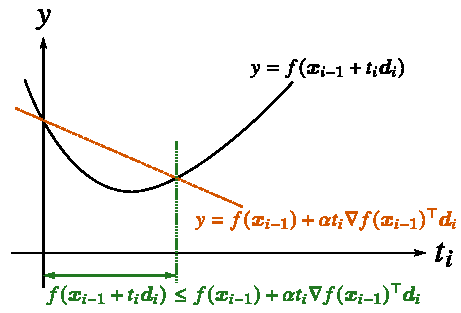
\includegraphics[width=0.7\linewidth]{optimization/Armijo-rule-image.pdf}
    \caption{Armijo の条件(式\eqref{optimization_unconstrained_descent-methods_Armijo-rule})のイメージ}
    \label{fig::optimization_unconstrained_descent-methods_Armijo-rule-image}
\end{figure}

Backtracking Line Search \cite[Section 9.2]{Boyd2004} は
Armijo の条件 \cite[Section 7.5]{Luenberger2003}
\begin{equation}
    f(\bm{x}_{i-1} + t_i \bm{d}_i) \le f(\bm{x}_{i-1}) + \alpha t_i \nabla f(\bm{x}_{i-1})^\top \bm{d}_i
    \label{eq:optimization_unconstrained_descent-methods_Armijo-rule}
\end{equation}
を利用する.
ここで,$\alpha$ は $\alpha \in (0,1)$ を満たす定数であり,
Armijo の条件は,
図\ref{fig:optimization_unconstrained_descent-methods_Armijo-rule-image}のように
十分小さい $t_i$ を選択するための条件となっている.
Backtracking Line Search では,
$\alpha \in (0, 1/2)$ とし,
Algorithm \ref{alg:optimization_unconstrained_descent-methods_BacktrackingLineSearch}
のように
$t_i$ を初期値 1 から $\beta \in (0, 1)$ 倍していき,
式 \eqref{eq:optimization_unconstrained_descent-methods_Armijo-rule} を満たすものを探索する.
一般に,パラメータ $\alpha$, $\beta$ は
$\alpha \in [0.01, 0.3]$, $\beta \in [0.1, 0.8]$ の範囲で設定される
\cite[Section 9.2]{Boyd2004}.

\subsection{最急降下法}

最急降下法では,更新方向を $\bm{d}_i = -\nabla f(\bm{x}_{i-1})$ とする.
確実に目的関数の減少する方向を示しており,
ここで示す他のアルゴリズムよりも更新方向の算出が簡単である.
目的関数が強凸関数である場合において,
最適解への収束が証明されている
\cite[Section 9.3.1]{Boyd2004}.

\subsection{Newton 法}

Newton 法では,
目的関数が狭義凸関数である(つまり,Hessian $\nabla^2 f(\bm{x}_{i-1})$ が正定値である)場合を対象とし,
更新方向を
$\bm{d}_i = -\nabla^2 f(\bm{x}_{i-1})^{-1} \nabla f(\bm{x}_{i-1})$
とする.
$\nabla^2 f(\bm{x}_{i-1})$ が正定値である場合,
$\nabla^2 f(\bm{x}_{i-1})^{-1}$ も正定値になる
\footnote{%
対称行列 $A$ が正定値である場合,$A$ の固有値は正の実数である.%
$A$ は固有値分解により $A=VDV^\top$ ($D$ は固有値による対角行列,$V$ は直交行列)と書くことができるため,%
$A^{-1} = VD^{-1}V^\top$ となる.%
よって,$A^{-1}$ の固有値も全て正の実数であり,%
$A^{-1}$ は正定値である.%
}
ため,
最適解でない $\bm{x}_{i-1}$ においては
$\nabla f(\bm{x}_{i-1})^\top \bm{d}_i = -\nabla f(\bm{x}_{i-1})^\top \nabla^2 f(\bm{x}_{i-1})^{-1} \nabla f(\bm{x}_{i-1}) < 0$
となり,目的関数が減少する方向になっていることを確認できる.
Newton 法の収束性については \cite[Section 9.5.3, 9.6.4]{Boyd2004} にて議論されている.

\subsection{準 Newton 法}

Newton 法では,
Hessian $\nabla^2 f(\bm{x}_{i-1})$ の逆行列が必要になるが,
$x^4$ のように 2 階微分が 0 になる点があったり,
Hessian の逆行列を安定的に計算できない点があったりする場合には使用できない.
そこで,Newton 法の更新方向
$\bm{d}_i = -\nabla^2 f(\bm{x}_{i-1})^{-1} \nabla f(\bm{x}_{i-1})$
における Hessian を
$\bm{d}_i = -H_{i-1} \nabla f(\bm{x}_{i-1})$
のように Hessian の代わりの行列で置き換える準 Newton 法と呼ばれるアルゴリズムがある.

準 Newton 法のうち,
Davidon-Fletcher-Powell (DFP) 公式では次のように $H_i$ を算出する
\cite[Section 9.3]{Luenberger2003}, \cite[Section 10.9]{Press2007}.
\begin{align}
    H_{i+1} &= H_i + \frac{\bm{p}_i \bm{p}_i^\top}{\bm{p}_i^\top \bm{q}_i}
        - \frac{H_i \bm{q}_i \bm{q}_i^\top H_i}{\bm{q}_i^\top H_i \bm{q}_i} \\
    \bm{p}_i &= \bm{x}_{i+1} - \bm{x}_i \\
    \bm{q}_i &= \nabla f(\bm{x}_{i+1}) - \nabla f(\bm{x}_i)
\end{align}
初期値 $H_0$ を対称な正定値の行列にしておけば,
全ての $H_i$ が帰納的に正定値になる
\cite[Section 9.3]{Luenberger2003}.
$H_i$ が正定値であれば,更新方向 $\bm{d}_i$ は目的関数の減少する方向になる.

また,同様の性質を持つ公式の 1 つとして,
Broyden-Fletcher-Goldfarb-Shanno (BFGS) 公式が存在する
\cite[Section 9.4]{Luenberger2003}.
\begin{align}
    H_i &= B_i^{-1} \\
    B_{i+1} &= B_i + \frac{\bm{q}_i \bm{q}_i^\top}{\bm{q}_i^\top \bm{p}_i}
        - \frac{B_i \bm{p}_i \bm{p}_i^\top B_i}{\bm{p}_i^\top B_i \bm{p}_i}
\end{align}
逆行列を計算することで次のようにも書くことができる
\cite[Section 10.9]{Press2007}.
\begin{align}
    H_{i+1} &= H_i + \frac{\bm{p}_i \bm{p}_i^\top}{\bm{p}_i^\top \bm{q}_i}
        - \frac{H_i \bm{q}_i \bm{q}_i^\top H_i}{\bm{q}_i^\top H_i \bm{q}_i}
        + \bm{q}_i^\top H_i \bm{q}_i \bm{v}_i \bm{v}_i^\top \\
    \bm{v}_i &= \frac{\bm{p}_i}{\bm{p}_i^\top \bm{q}_i}
        - \frac{H_i \bm{q}_i}{\bm{q}_i^\top H_i \bm{q}_i}
\end{align}

\subsection{共役勾配法}

共役勾配法では,
\begin{align}
    \bm{d}_1 &= -\nabla f(\bm{x}_{i-1}) \\
    \bm{d}_i &= -\nabla f(\bm{x}_{i-1}) + \gamma_i \bm{d}_{i-1} \\
    \gamma_i &= 
        \frac{(\nabla f(\bm{x}_{i-1}) - \nabla f(\bm{x}_{i-2}))^\top \nabla f(\bm{x}_{i-1})}
        {\|\nabla f(\bm{x}_{i-2})\|_2^2}
\end{align}
のように更新方向を算出する
\cite[Section 8.6]{Luenberger2003}.
$\gamma_i$ については複数の形式があるが,
ここで示している Polak-Ribiere 法は一般により良い結果が得られるという
\cite[Section 8.6]{Luenberger2003}, \cite[Section 10.8]{Press2007}.
Newton 法では計算量の多い逆行列の計算が必要だが,
共役勾配法では計算量が変数の次元のオーダーに収まるため,
各反復の計算時間を抑えられる.



% !TEX root = ../main.tex
%

\part{求根アルゴリズム}

\chapter{導入}

求根アルゴリズム (root-finding algorithm)
は,微分などの演算を含まない通常の方程式
$f(\bm{x})=\bm{0}$ ($f : \setR^n \to \setR^m$)
の解を求めるためのアルゴリズムである.
関数 $f$ の種類に依り様々な手法が存在する.

\chapter{記号}

本部で使用する記号を以下に示す.

\begin{explainlist}
    $\setR$ & 実数の集合 \\
    $f'(x)$ & 1 変数関数 $f : \setR \to \setR$ の微分係数 \\
    $\nabla f$ & 関数 $f : \setR^n \to \setR$ の勾配 \\
    $\frac{\partial \bm{f}}{\partial \bm{x}}$ & 関数 $\bm{f} : \setR^n \to \setR^n$ の Jacobian \\
    $\|\bm{x}\|_2$ & ベクトル $\bm{x}$ の 2-ノルム \\
\end{explainlist}

% !TEX root = ../main.tex
%

\chapter{Newton-Raphson 法}\label{chap:root-finding_newton-raphson}

Newton-Raphson 法は,
次の式のような更新式で反復的に方程式 $f(x) = 0$ の根を求める手法である.
\begin{equation}
    x_{n+1} = x_n - \frac{f(x_n)}{f'(x_n)}
\end{equation}

\section{1 次元の方程式の場合}

1 次元の方程式 $f(x) = 0$ ($f: \setR \to \setR$) の場合,
1 次近似
\begin{equation}
    f(x_{n+1}) \approx f(x_n) + f'(x_n) (x_{n+1} - x_n)
\end{equation}
の根を求めると
\begin{equation}
    x_{n+1} = x_n - \frac{f(x_n)}{f'(x_n)}
    \label{eq:root-finding_newton-raphson_one-dim-update-law}
\end{equation}
と更新式が導かれる.

\subsection{平方根の算出}

ここでは,平方根の算出に Newton-Raphson 法を適用してみる.

$a>0$ について $\sqrt{a}$ を算出する場合,次の関数 $f$ の正の根を求めれば良い.
\begin{equation}
    f(x) = x^2 - a
\end{equation}
この関数を微分すると
\begin{equation}
    f'(x) = 2x
\end{equation}
となる.
よって,更新式は次のようになる.
\begin{align}
    x_{n+1} & = x_n - \frac{f(x_n)}{f'(x_n)}          \notag \\
            & = x_n - \frac{x_n^2 - a}{2x_n}          \notag \\
            & = \frac{1}{2}\left(x_n + \frac{a}{x_n}\right)
    \label{eq:root-finding_newton-raphson_sqrt-update-law}
\end{align}

\begin{theorem}
    式 \eqref{eq:root-finding_newton-raphson_sqrt-update-law} の更新式は,
    初期値 $x_0$ が $x_0 > 0$ を満たす場合,
    平方根 $\sqrt{a}$ に収束する.
\end{theorem}
\begin{proof}
    $x_0 = \sqrt{a}$ の場合は
    $k = 1, 2, \ldots$ において $x_k = \sqrt{a}$ が成り立つ.
    つまり,平方根 $\sqrt{a}$ に収束している.
    そこで,以下では $x_0 \neq \sqrt{a}$ とする.

    更新後の値 $x_{n+1}$ と平方根 $\sqrt{a}$ の差は次のようになる.
    \begin{align}
          & x_{n+1} - \sqrt{a}                                                      \notag \\
        = & \frac{1}{2} (x_n - \sqrt{a}) + \frac{1}{2} \frac{a - \sqrt{a} x_n}{x_n} \notag \\
        = & \frac{1}{2} (x_n - \sqrt{a}) \left(1 - \frac{\sqrt{a}}{x_n}\right)      \notag \\
        = & \frac{1}{2x_n} (x_n - \sqrt{a})^2
        \label{eq:root-finding_newton-raphson_sqrt-error-update}
    \end{align}

    $x_0 > 0$ かつ $x_0 \neq \sqrt{a}$ の場合,
    式 \eqref{eq:root-finding_newton-raphson_sqrt-error-update} より
    $x_1 - \sqrt{a} > 0$ が成り立つ.
    さらに,$k = 2, 3, \ldots$ において $x_k - \sqrt{a} > 0$ であることも帰納的に成り立つ.
    よって,$k = 1, 2, \ldots$ において $x_k - \sqrt{a} > 0$ である.

    また,$a > 0$ より $\sqrt{a} > 0$ であることを用いると,
    \begin{align}
          & x_{n+1} - \sqrt{a}                           \notag \\
        = & \frac{1}{2x_n} (x_n - \sqrt{a})^2            \notag \\
        = & \frac{x_n - \sqrt{a}}{2x_n} (x_n - \sqrt{a}) \notag \\
        < & \frac{x_n}{2x_n} (x_n - \sqrt{a})            \notag \\
        = & \frac{1}{2} (x_n - \sqrt{a})
    \end{align}
    となる.

    以上から,
    \begin{equation}
        0 < x_{n+1} - \sqrt{a} < \frac{1}{2} (x_n - \sqrt{a})
    \end{equation}
    が成り立ち,$x_n$ の列が平方根 $\sqrt{a}$ へ収束する.
\end{proof}

\subsection{べき根の算出}

一般に $r$ 乗根($r = 2, 3, \ldots$)を算出することを考える.

$a>0$ について $\sqrt[r]{a}$ を算出する場合,次の関数 $f$ の正の根を求めれば良い.
\begin{equation}
    f(x) = x^r - a
\end{equation}
この関数を微分すると
\begin{equation}
    f'(x) = rx^{r-1}
\end{equation}
となる.
よって,更新式は次のようになる.
\begin{align}
    x_{n+1} & = x_n - \frac{f(x_n)}{f'(x_n)}             \notag \\
            & = x_n - \frac{x_n^r - a}{rx_n^{r-1}}       \notag \\
            & = \frac{r-1}{r} x_n + \frac{a}{rx_n^{r-1}}
    \label{eq:root-finding_newton-raphson_rth-root-update-law}
\end{align}

\begin{theorem}
    式 \eqref{eq:root-finding_newton-raphson_rth-root-update-law} の更新式は,
    初期値 $x_0$ が $x_0 > 0$ を満たす場合,
    べき根 $\sqrt[r]{a}$ に収束する.
\end{theorem}
\begin{proof}
    $x_0 = \sqrt[r]{a}$ の場合は
    $k = 1, 2, \ldots$ において $x_k = \sqrt[r]{a}$ が成り立つ.
    つまり,平方根 $\sqrt[r]{a}$ に収束している.
    そこで,以下では $x_0 \neq \sqrt[r]{a}$ とする.

    更新後の値 $x_{n+1}$ とべき根 $\sqrt[r]{a}$ の差は次のようになる.
    \begin{align}
          & x_{n+1} - \sqrt[r]{a}                                    \notag \\
        = & \frac{r-1}{r} \left(x_n - \sqrt[r]{a}\right)
        + \frac{1}{r} \left(\frac{a}{x_n^{r-1}} - \sqrt[r]{a}\right) \notag \\
        = & \frac{r-1}{r} \left(x_n - \sqrt[r]{a}\right)
        -\frac{\sqrt[r]{a}}{r} \left(1 - \left(\frac{\sqrt[r]{a}}{x_n}\right)^{r-1}\right)
    \end{align}
    これに等比級数の公式
    \begin{equation}
        \sum_{k = 1}^n x^{k-1} = \frac{1 - x^n}{1 - x}
    \end{equation}
    を適用すると,
    \begin{align}
          & x_{n+1} - \sqrt[r]{a}                                                \notag     \\
        = & \frac{r-1}{r} \left(x_n - \sqrt[r]{a}\right)
        -\frac{\sqrt[r]{a}}{r} \left(1 - \frac{\sqrt[r]{a}}{x_n}\right)
        \sum_{k = 1}^{r - 1} \left(\frac{\sqrt[r]{a}}{x_n}\right)^{k - 1}        \notag     \\
        = & \frac{r-1}{r} \left(x_n - \sqrt[r]{a}\right)
        -\frac{1}{r} \left(x_n - \sqrt[r]{a}\right)
        \sum_{k = 1}^{r - 1} \left(\frac{\sqrt[r]{a}}{x_n}\right)^k              \notag     \\
        = & \frac{1}{r} \left(x_n - \sqrt[r]{a}\right)
        \left(r - 1 - \sum_{k = 1}^{r - 1} \left(\frac{\sqrt[r]{a}}{x_n}\right)^k\right)
        \label{eq:root-finding_newton-raphson_rth-root-error-update-linear}                 \\
        = & \frac{1}{r} \left(x_n - \sqrt[r]{a}\right)
        \sum_{k = 1}^{r - 1} \left(1 - \left(\frac{\sqrt[r]{a}}{x_n}\right)^k\right) \notag \\
        = & \frac{1}{r} \left(x_n - \sqrt[r]{a}\right)
        \left(1 - \frac{\sqrt[r]{a}}{x_n}\right)
        \sum_{k = 1}^{r - 1} \sum_{l = 1}^{k}
        \left(\frac{\sqrt[r]{a}}{x_n}\right)^{l - 1}                                 \notag \\
        = & \frac{1}{rx_n} \left(x_n - \sqrt[r]{a}\right)^2
        \sum_{k = 1}^{r - 1} \sum_{l = 1}^{k}
        \left(\frac{\sqrt[r]{a}}{x_n}\right)^{l - 1}
        \label{eq:root-finding_newton-raphson_rth-root-error-update-quadratic}
    \end{align}
    となる.

    $x_0 > 0$ かつ $x_0 \neq \sqrt[r]{a}$ の場合,
    式 \eqref{eq:root-finding_newton-raphson_rth-root-error-update-quadratic} より
    $x_1 - \sqrt[r]{a} > 0$ が成り立つ.
    さらに,$k = 2, 3, \ldots$ において $x_k - \sqrt[r]{a} > 0$ であることも帰納的に成り立つ.
    よって,$k = 1, 2, \ldots$ において $x_k - \sqrt[r]{a} > 0$ である.

    さらに,$x_n > \sqrt[r]{a} > 0$ であることから
    $\sqrt[r]{a} / x_n > 0$ が成り立つから,
    式 \eqref{eq:root-finding_newton-raphson_rth-root-error-update-linear} より
    \begin{align}
          & x_{n+1} - \sqrt[r]{a}                          \notag \\
        < & \frac{r - 1}{r} \left(x_n - \sqrt[r]{a}\right)
    \end{align}
    となる.

    以上から,
    \begin{equation}
        0 < x_{n+1} - \sqrt[r]{a} < \frac{r - 1}{r} \left(x_n - \sqrt[r]{a}\right)
        \label{eq:root-finding_newton-raphson_rth-root-error-convergence}
    \end{equation}
    が成り立ち,$x_n$ の列がべき根 $\sqrt[r]{a}$ へ収束する.
\end{proof}

$r$ が奇数の場合,
負の数 $a < 0$ に対してべき根 $\sqrt[r]{a} < 0$ が存在する.
この場合についてもべき根の算出を考える.

\begin{theorem}
    $r = 3, 5, 7, \ldots$ かつ $a < 0$ の場合を考える.
    式 \eqref{eq:root-finding_newton-raphson_rth-root-update-law} の更新式は,
    初期値 $x_0$ が $x_0 < 0$ を満たす場合,
    べき根 $\sqrt[r]{a}$ に収束する.
\end{theorem}
\begin{proof}
    $x_0 = \sqrt[r]{a}$ の場合は
    $k = 1, 2, \ldots$ において $x_k = \sqrt[r]{a}$ が成り立つ.
    つまり,平方根 $\sqrt[r]{a}$ に収束している.
    そこで,以下では $x_0 \neq \sqrt[r]{a}$ とする.

    $x_0 < 0$ かつ $x_0 \neq \sqrt[r]{a}$ の場合,
    式 \eqref{eq:root-finding_newton-raphson_rth-root-error-update-quadratic} より
    $x_1 - \sqrt[r]{a} < 0$ が成り立つ.
    さらに,$k = 2, 3, \ldots$ において $x_k - \sqrt[r]{a} < 0$ であることも帰納的に成り立つ.
    よって,$k = 1, 2, \ldots$ において $x_k - \sqrt[r]{a} < 0$ である.

    さらに,$x_n < \sqrt[r]{a} < 0$ であることから
    $\sqrt[r]{a} / x_n > 0$ が成り立つから,
    式 \eqref{eq:root-finding_newton-raphson_rth-root-error-update-linear} より
    \begin{align}
          & x_{n+1} - \sqrt[r]{a}                          \notag \\
        > & \frac{r - 1}{r} \left(x_n - \sqrt[r]{a}\right)
    \end{align}
    となる.

    以上から,
    \begin{equation}
        \frac{r - 1}{r} \left(x_n - \sqrt[r]{a}\right) < x_{n+1} - \sqrt[r]{a} < 0
    \end{equation}
    が成り立ち,$x_n$ の列がべき根 $\sqrt[r]{a}$ へ収束する.
\end{proof}

\section{2 次元以上の方程式の場合}

一般に $n$ 次元($n=1,2,\ldots$)の方程式
$\bm{f}(\bm{x}) = \bm{0}$ ($\bm{f}: \setR^n \to \setR^n$) の場合,
1 次近似
\begin{equation}
    \bm{f}(\bm{x}_{n+1}) \approx
    \bm{f}(\bm{x}_n) + \frac{\partial \bm{f}}{\partial \bm{x}} (\bm{x}_{n+1} - \bm{x}_n)
\end{equation}
をもとに更新式
\begin{equation}
    \bm{x}_{n+1} = \bm{x}_n - \left(\frac{\partial \bm{f}}{\partial \bm{x}}\right)^{-1} \bm{f}(\bm{x}_n)
\end{equation}
が得られる.


% !TEX root = ../main.tex
%

\part{常微分方程式の数値解法}

\chapter{導入}

\index{じょうびぶんほうていしき@常微分方程式}
\index{ordinary differential equation|see{常微分方程式}}
この部では,常微分方程式 (ordinary differential equation, ODE) の数値解法をまとめる.

関数 $\bm{y}(t)$ の常微分方程式は一般に
\begin{equation}
    \bm{f}(t, \bm{y}, \dot{\bm{y}}, \ddot{\bm{y}}, \dddot{\bm{y}}, \ddddot{\bm{y}}, \ldots) = \bm{0}
\end{equation}
のように書ける.

% !TEX root = ../main.tex
%

\chapter{Runge-Kutta 法}

Runge-Kutta 法 (Runge-Kutta method) では次のような形式の初期値問題を数値的に解く
\cite{Mitsui1993}.
\begin{equation}
    \begin{cases}
        \dot{\bm{y}} = \bm{f}(t, \bm{y}) \\
        \bm{y}(0) = \bm{y}_0
    \end{cases}
\end{equation}

Runge-Kutta 法は,時刻 $t$ における変数 $\bm{y}(t)$ の値から,
次のような形式で時刻 $t + h$ における変数 $\bm{y}(t + h)$ の計算を行う.
\begin{align}
    \bm{k}_i      & = \bm{f}\left(t + c_i h, \bm{y}(t) + h \sum_{j = 1}^s a_{ij} \bm{k}_j \right)
                  & \text{for $i = 1, 2, \ldots, s$}
    \label{eq:ode_runge-kutta_k-law}                                                              \\
    \bm{y}(t + h) & = \bm{y}(t) + \sum_{i=1}^s b_i \bm{k}_i
    \label{eq:ode_runge-kutta_y-law}
\end{align}

ここで,時間の更新幅 $h$ はステップ幅と呼ばれる.
Runge-Kutta 法には,
整数 $s$ (段数と呼ばれる)と係数 $a_{ij}$, $b_i$, $c_i$ の異なる様々な公式が存在する.
係数 $a_{ij}$, $b_i$, $c_i$ は
表 \ref{table:ode_runge-kutta_butcher-array-general} のような
Butcher 配列と呼ばれる形式で記載される.

\begin{table}[bp]
    \caption{Butcher 配列における係数の並べ方}
    \label{table:ode_runge-kutta_butcher-array-general}
    \centering
    \begin{tabular}{c|ccccc}
        $c_1$    & $a_{11}$ & $a_{12}$ & $a_{13}$ & $\cdots$ & $a_{1s}$ \\
        $c_2$    & $a_{21}$ & $a_{22}$ & $a_{23}$ & $\cdots$ & $a_{2s}$ \\
        $c_3$    & $a_{31}$ & $a_{32}$ & $a_{33}$ & $\cdots$ & $a_{3s}$ \\
        $\vdots$ & $\vdots$ & $\vdots$ & $\vdots$ & $\ddots$ & $\vdots$ \\
        $c_s$    & $a_{s1}$ & $a_{s2}$ & $a_{s3}$ & $\cdots$ & $a_{ss}$ \\
        \hline
                 & $b_1$    & $b_2$    & $b_3$    & $\cdots$ & $b_s$
    \end{tabular}
\end{table}

Runge-Kutta 法の公式は次のように分類される.

\begin{description}
    \item[陽的 Runge-Kutta 法] $j \ge i$ について $a_{ij} = 0$ となっている場合,
          $\bm{k}i$ は $\bm{k}_1, \bm{k}_2, \ldots, \bm{k}_s$
          の順に式 \eqref{eq:ode_runge-kutta_k-law} の右辺を評価することで計算できる.
          このような場合は陽的 Runge-Kutta 法と呼ばれる.
    \item[半陰的 Runge-Kutta 法] $j > i$ について $a_{ij} = 0$ となっている場合,
          $\bm{k}i$ は $\bm{k}_1, \bm{k}_2, \ldots, \bm{k}_s$
          の順に式 \eqref{eq:ode_runge-kutta_k-law} を $\bm{k}_i$ について解くことで計算できる.
          このような場合は半陰的 Runge-Kutta 法と呼ばれる.
    \item[陰的 Runge-Kutta 法] $j > i$ でも $a_{ij} \neq 0$ となる係数が存在する場合,
          $\bm{k}i$ は $i = 1, 2, \ldots, s$ について連立した
          式 \eqref{eq:ode_runge-kutta_k-law} を $\bm{k}_i$ について解くことで計算する.
          このような場合は陰的 Runge-Kutta 法と呼ばれる.
\end{description}

陽的 Runge-Kutta 法の方が計算は単純だが,
陰的 Runge-Kutta 法は

\begin{itemize}
    \item 硬い系と呼ばれる比較的不安定な微分方程式で解が安定しやすい.
    \item 陽的 Runge-Kutta 法よりも少ない段数でより高い次数を出せる.
          (後述する公式の実例を見ると分かる.)
\end{itemize}

といった利点を持つ.
そのため,解が安定するようにステップ幅を調整した場合,
陰的 Runge-Kutta 法の方がステップ幅を大きくとることができ,
目的の時刻 $t$ までの解を得るために必要な計算時間は少なくなる場合がある.

また,Runge-Kutta 法の公式の精度を示す数値として次数が存在する.
変数の近似値 $\bm{y}(t + h)$ の精度が $h^p$ オーダーの場合,
その公式は $p$ 次といい,$p$ は次数と呼ばれる.

\section{埋め込み型公式}

Runge-Kutta 法の公式の中には,複数の $b_i$ の組を持つものがある
(表 \ref{table:ode_runge-kutta_butcher-array-rkf45} の例を参照).
そのような公式では,次のような 2 つの近似値を得ることができる.
\begin{align}
    \bm{y}(t + h)   & = \bm{y}(t) + \sum_{i=1}^s b_i \bm{k}_i     \\
    \bm{y}^*(t + h) & = \bm{y}^*(t) + \sum_{i=1}^s b_i^* \bm{k}_i
\end{align}
これらの差により誤差の近似値を求めることができる.
\begin{align}
    \bm{y}(t + h) - \bm{y}^*(t + h) & = \sum_{i=1}^s (b_i - b_i^*) \bm{k}_i
\end{align}

これを用いると,現在のステップ幅から次のステップ幅 $\hat{h}$ の適正値を推定できる.
まず,$b_i$ と $b_i^*$ のうち次数が低い方の次数を $p$ とすると,
\begin{align}
    \left| \bm{y}(t + h) - \bm{y}^*(t + h) \right| \approx |Ah^p|
\end{align}
のように書ける.
そこで,誤差の許容量を $\epsilon_{tol}$ としたとき,次の方程式が成り立つようにする.
\begin{equation}
    \frac{\hat{h}^p}{h^p} = \frac{\epsilon_{tol}}{\left| \bm{y}(t + h) - \bm{y}^*(t + h) \right|}
\end{equation}
これを $\hat{h}$ について解くと,次のようになる.
\begin{equation}
    \hat{h} = h \left(\frac{\epsilon_{tol}}{\left| \bm{y}(t + h) - \bm{y}^*(t + h) \right|}\right)^{\frac{1}{p}}
\end{equation}

\section{古典的 Runge-Kutta 法}

\begin{table}[bp]
    \caption{古典的 Runge-Kutta 法 (RK4 公式)の Butcher 配列}
    \label{table:ode_runge-kutta_butcher-array-rk4}
    \centering
    \begin{tabular}{c|cccc}
        $0$           &               &               &               &               \\
        $\frac{1}{2}$ & $\frac{1}{2}$ &               &               &               \\
        $\frac{1}{2}$ & $0$           & $\frac{1}{2}$ &               &               \\
        $1$           & $0$           & $0$           & $1$           &               \\
        \hline
                      & $\frac{1}{6}$ & $\frac{1}{3}$ & $\frac{1}{3}$ & $\frac{1}{6}$
    \end{tabular}
\end{table}

古典的 Runge-Kutta 法と呼ばれる公式では,
表 \ref{table:ode_runge-kutta_butcher-array-rk4} のような係数を用いる
\cite[3.3 節]{Mitsui1993}.
単純な係数で次数 4 を達成できる.

\section{RKF45 公式}

\begin{table}[bp]
    \caption{RKF45 公式の Butcher 配列}
    \label{table:ode_runge-kutta_butcher-array-rkf45}
    \centering
    \begin{tabular}{c|ccccccc}
        $0$             &                     &                      &                      &                       &                  &                &          \\
        $\frac{1}{4}$   & $\frac{1}{4}$       &                      &                      &                       &                  &                &          \\
        $\frac{3}{8}$   & $\frac{3}{32}$      & $\frac{9}{32}$       &                      &                       &                  &                &          \\
        $\frac{12}{13}$ & $\frac{1932}{2197}$ & $-\frac{7200}{2197}$ & $\frac{7296}{2197}$  &                       &                  &                &          \\
        $1$             & $\frac{439}{216}$   & $-8$                 & $\frac{3680}{513}$   & $-\frac{845}{4104}$   &                  &                &          \\
        $\frac{1}{2}$   & $-\frac{8}{27}$     & $2$                  & $-\frac{3544}{2565}$ & $\frac{1859}{4104}$   & $-\frac{11}{40}$ &                &          \\
        \hline
                        & $\frac{16}{135}$    & $0$                  & $\frac{6656}{12825}$ & $\frac{28561}{56430}$ & $-\frac{9}{50}$  & $\frac{2}{55}$ & (5 次) \\
                        & $\frac{25}{216}$    & $0$                  & $\frac{1408}{2565}$  & $\frac{2197}{4104}$   & $-\frac{1}{5}$   & $0$            & (4 次)
    \end{tabular}
\end{table}

RKF45 公式(RKF は Runge-Kutta-Fehlberg のこと)では,
表 \ref{table:ode_runge-kutta_butcher-array-rkf45} のような係数を用いる
\cite[4.1 節 (a)]{Mitsui1993}, \cite[Section 9.5]{Mathews2004}.
この埋め込み型公式では,$\bm{k}_i$ から $\bm{y}(t + h)$ を算出する係数に
5 次の精度を持つ組と 4 次の精度を持つ組が存在する
\footnote{挙げた 2 件の文献のうち,%
    文献 \cite{Mitsui1993} では係数が一カ所誤っていたため注意が必要.}.

\section{田中公式}

\begin{table}[bp]
    \caption{田中 Formula1 公式の Butcher 配列}
    \label{table:ode_runge-kutta_butcher-array-tanaka-formula1}
    \centering
    \begin{tabular}{c|ccc}
        $\frac{13}{20}$ & $\frac{13}{20}$    &                  &          \\
        $-\frac{1}{18}$ & $-\frac{127}{180}$ & $\frac{13}{20}$  &          \\
        \hline
                        & $\frac{100}{127}$  & $\frac{27}{127}$ & (3 次) \\
                        & $1$                &                  & (1 次)
    \end{tabular}
\end{table}

\begin{table}[bp]
    \caption{田中 Formula2 公式の Butcher 配列}
    \label{table:ode_runge-kutta_butcher-array-tanaka-formula2}
    \centering
    \begin{tabular}{c|cccc}
        $\frac{133}{100}$ & $\frac{133}{100}$     &                       &                      &          \\
        $\frac{1}{2}$     & $-\frac{5400}{18167}$ & $\frac{28967}{36334}$ &                      &          \\
        $-\frac{33}{100}$ & $\frac{133}{50}$      & $-\frac{108}{25}$     & $\frac{133}{100}$    &          \\
        \hline
                          & $\frac{1250}{20667}$  & $\frac{18167}{20667}$ & $\frac{1250}{20667}$ & (4 次) \\
                          & $0$                   & $1$                   &                      & (2 次)
    \end{tabular}
\end{table}

文献 \cite{Togawa2007} では,田中正次氏が考案した半陰的・陰的公式がいくつか示されている.
そのうち埋め込み型の半陰的公式を表
\ref{table:ode_runge-kutta_butcher-array-tanaka-formula1},
\ref{table:ode_runge-kutta_butcher-array-tanaka-formula2}
に示す
\footnote{文献 \cite{Togawa2007} には完全に陰的な 4 段 7 次の公式もあるが,%
    係数がかなり複雑なため省略した.}.

段数の多い陽的公式と同程度の精度を少ない段数で出すことができていることを確認できる.
また,埋め込み型の 2 つの係数のうち次数の低い方の係数が単純になっている
\footnote{利用する際には高い次数の係数との差を見るように実装するため,%
    次数の低い方の係数だけ単純でも計算コストへの影響はない.}.

\section{Butcher-Kuntzmann 公式}

\begin{table}[bp]
    \caption{2 段 Butcher-Kuntzmann 公式の Butcher 配列}
    \label{table:ode_runge-kutta_butcher-array-2stage-butcher-kuntzmann}
    \centering
    \begin{tabular}{c|cc}
        $\frac{1}{2} + \frac{\sqrt{3}}{6}$ & $\frac{1}{4}$                      & $\frac{1}{4} + \frac{\sqrt{3}}{6}$ \\
        $\frac{1}{2} - \frac{\sqrt{3}}{6}$ & $\frac{1}{4} - \frac{\sqrt{3}}{6}$ & $\frac{1}{4}$                      \\
        \hline
                                           & $\frac{1}{2}$                      & $\frac{1}{2}$
    \end{tabular}
\end{table}

文献 \cite[5.2 節 (b)]{Mitsui1993} によると,
陰的 Runge-Kutta 法では,$s$ 段公式で $2s$ 次を超えることができないと証明されており,
その限界の $2s$ 次の公式が存在することも証明されている.
特に Legendre 関数の零点を用いて係数を決める種類の公式は,
$s$ 段 Butcher-Kuntzmann 公式と呼ばれる.
2 段 Butcher-Kuntzmann 公式を表
\ref{table:ode_runge-kutta_butcher-array-2stage-butcher-kuntzmann}
に示す(前述の通り 4 次の精度を持つ).

\section{Euler 法}

\begin{table}[bp]
    \caption{Euler 法の Butcher 配列}
    \label{table:ode_runge-kutta_butcher-array-explicit-euler}
    \centering
    \begin{tabular}{c|c}
        $1$ &     \\
        \hline
            & $1$
    \end{tabular}
\end{table}

常微分方程式の解法としては最も基本的な Euler 法
\begin{equation}
    \bm{y}(t + h) \approx \bm{y}(t) + h \bm{f}(t, \bm{y}(t))
\end{equation}
は形式的に Runge-Kutta 法とみなすことができる.
Butcher 配列は表 \ref{table:ode_runge-kutta_butcher-array-explicit-euler} に示す通りである.

% !TEX root = ../main.tex
%

\chapter{平均ベクトル場法}

エネルギー保存則を満たす系の運動方程式を解くことを目的とした手法の 1 つとして,
平均ベクトル場法(Average vector field method, AVF method) \cite{Quispel2008} がある.

座標 $\bm{q}$ に対して,
運動エネルギーが $T = \bm{p}^\top \dot{\bm{q}} / 2$ で表現されるようにモーメント $\bm{p}$ を定める.
さらに位置エネルギー $V$ を座標 $\bm{q}$ で表現することで,
全エネルギーの和を表現した関数 $H(\bm{q}, \bm{p}) = T + V$ を
ハミルトニアン(Hamiltonian)と呼ぶ
\cite[Section 3.2]{Morse1953}.
このとき,運動方程式は次の式で表現される.
\begin{align}
    \dot{\bm{q}} & = \frac{\partial H}{\partial \bm{p}}  \\
    \dot{\bm{p}} & = -\frac{\partial H}{\partial \bm{q}}
\end{align}
この式は変数 $\bm{y} = (\bm{q}^\top, \bm{p}^\top)^\top$ を用いて次のように書くこともできる.
\begin{equation}
    \dot{\bm{y}} = \bm{f}(\bm{y}) \equiv S \nabla H(\bm{y})
\end{equation}
文献 \cite{Quispel2008} はこの形式の微分方程式を前提として
次のような数値解法を提案している.
\begin{equation}
    \frac{\bm{y}_{n+1} - \bm{y}_n}{h}
    = \int_{0}^{1} \bm{f}((1 - \xi) \bm{y}_n + \xi \bm{y}_{n+1}) d \xi
    \label{eq:ode_average-vector-field_update-2-order}
\end{equation}

この手法がエネルギーを保存することを示す.
まず,$\bm{f}(\bm{y}) \equiv S \nabla H(\bm{y})$ より
\begin{equation}
    \frac{\bm{y}_{n+1} - \bm{y}_n}{h}
    = S \int_{0}^{1} \nabla H((1 - \xi) \bm{y}_n + \xi \bm{y}_{n+1}) d \xi
    \label{eq:ode_average-vector-field_update-with-hamiltonian}
\end{equation}
である.ここで,$S$ は
\begin{equation}
    S =
    \begin{pmatrix}
        O  & I \\
        -I & O
    \end{pmatrix}
\end{equation}
であるため
\footnote{このような行列は歪対称行列と呼ばれる.}
,任意のベクトル $\bm{y} = (\bm{q}^\top, \bm{p}^\top)^\top$ において,
\begin{equation}
    \bm{y}^\top S \bm{y} =
    \begin{pmatrix}
        \bm{q}^\top & \bm{p}^\top
    \end{pmatrix}
    \begin{pmatrix}
        O  & I \\
        -I & O
    \end{pmatrix}
    \begin{pmatrix}
        \bm{q} \\ \bm{p}
    \end{pmatrix}
    =
    \begin{pmatrix}
        \bm{q}^\top & \bm{p}^\top
    \end{pmatrix}
    \begin{pmatrix}
        \bm{p} \\ -\bm{q}
    \end{pmatrix}
    = \bm{0}
\end{equation}
となる.よって,
式 \eqref{eq:ode_average-vector-field_update-with-hamiltonian}
の両辺と
$\int_{0}^{1} \nabla H((1 - \xi) \bm{y}_n + \xi \bm{y}_{n+1}) d \xi$ の内積をとると
\begin{equation}
    \frac{\bm{y}_{n+1} - \bm{y}_n}{h}
    \int_{0}^{1} \nabla H((1 - \xi) \bm{y}_n + \xi \bm{y}_{n+1}) d \xi
    = 0
\end{equation}
となる.さらに左辺は
\begin{align}
      & \frac{\bm{y}_{n+1} - \bm{y}_n}{h}
    \int_{0}^{1} \nabla H((1 - \xi) \bm{y}_n + \xi \bm{y}_{n+1}) d \xi         \\
    = & \frac{1}{h}
    \int_{0}^{1} \frac{d}{d\xi} H((1 - \xi) \bm{y}_n + \xi \bm{y}_{n+1}) d \xi \\
    = & \frac{H(\bm{y}_{n+1}) - H()\bm{y}_{n})}{h}
\end{align}
と変形できるから,次のようにエネルギーの保存が示される.
\begin{equation}
    H(\bm{y}_{n+1}) - H(\bm{y}_{n}) = 0
\end{equation}

式 \eqref{eq:ode_average-vector-field_update-2-order} は 2 次の精度だが,
3 次と 4 次の公式も文献 \cite{Quispel2008} で示されている.
それらは次の式で与えられる.
\begin{equation}
    \frac{\bm{y}_{n+1} - \bm{y}_n}{h}
    = \left(I + \alpha h^2
    \left(\left. \frac{\partial \bm{f}}{\partial \bm{y}} \right|_{\bm{y} = \hat{\bm{y}}}\right)^2
    \right)
    \int_{0}^{1} \bm{f}((1 - \xi) \bm{y}_n + \xi \bm{y}_{n+1}) d \xi
\end{equation}
パラメータと次数は次のようになる.
\begin{itemize}
    \item $\alpha = 0$ とすると 2 次精度の更新式
          \eqref{eq:ode_average-vector-field_update-2-order}
          が得られる.
    \item $\alpha = -1/12$, $\hat{\bm{y}} = \bm{y}_n$ とすると
          3 次精度の更新式が得られる.
    \item $\alpha = -1/12$, $\hat{\bm{y}} = (\bm{y}_n + \bm{y}_{n+1})/2$ とすると
          4 次精度の更新式が得られる.
\end{itemize}

この手法の更新式は次数に依らず陰的で,
次数が上がるごとに計算が複雑になっていく.
ここで,次数 2 のときの方程式
\begin{equation}
    F(\bm{y}_{n+1}) \equiv
    \frac{\bm{y}_{n+1} - \bm{y}_n}{h} -
    \int_{0}^{1} \bm{f}((1 - \xi) \bm{y}_n + \xi \bm{y}_{n+1}) d \xi
    = 0
\end{equation}
を考える.
これを Newton-Raphson 法(\ref{chap:root-finding_newton-raphson} 章)で解くには,
Jacobian が必要となる.
Jacobian は次のようになる.
\begin{equation}
    \frac{\partial F}{\partial \bm{y}_{n+1}} =
    \frac{1}{h} I -
    \int_{0}^{1} \xi \left. \frac{\partial \bm{f}}{\partial \bm{y}} \right|_{\bm{y} = (1 - \xi) \bm{y}_n + \xi \bm{y}_{n+1}} d \xi
\end{equation}
さらに,Jacobian の変化が十分小さいとすると,
\begin{align}
            & \frac{\partial F}{\partial \bm{y}_{n+1}}                                                \\
    \approx & \frac{1}{h} I -
    \int_{0}^{1} \xi \left. \frac{\partial \bm{f}}{\partial \bm{y}} \right|_{\bm{y} = \bm{y}_n} d \xi \\
    =       & \frac{1}{h} I - \frac{1}{2}
    \left. \frac{\partial \bm{f}}{\partial \bm{y}} \right|_{\bm{y} = \bm{y}_n}
    \label{eq:ode_average-vector-field_approx-jacobian}
\end{align}
のように近似できる.
3 次と 4 次の更新式でも,Newton-Raphson 法の Jacobian においては $h^2$ の項を無視して
式 \eqref{eq:ode_average-vector-field_approx-jacobian} で
近似することができる.


% !TEX root = ../main.tex
%

\part{高精度演算}

% !TEX root = ../main.tex
%

\chapter{倍精度浮動小数点数による多倍長浮動小数点数}

倍精度浮動小数点数を用いて四倍精度,八倍精度といったより高い精度の演算を行う手法が考えられている
\cite{Hirayama2014,Hida2001}.
それぞれ 2 つ,4 つの倍精度浮動小数点数の和で小数を表現し,
仮数の桁が被らないように演算することで高い精度を実現する.

\section{記号}

本章で使用する記号を以下に示す.

\begin{explainlist}
    $\oplus$ & 倍精度浮動小数点数の加算 \\
    $\ominus$ & 倍精度浮動小数点数の減算 \\
    $\otimes$ & 倍精度浮動小数点数の乗算 \\
    $\oslash$ & 倍精度浮動小数点数の除算 \\
\end{explainlist}

\section{基本演算}

倍精度浮動小数点数による四倍精度,八倍精度演算の既存文献\cite{Hida2001}で使用される
基本的な演算を以下にまとめる.

まず,$|a| \ge |b|$ となる倍精度浮動小数点数 $a$, $b$ について
$s = a \oplus b$, $a + b = s + e$ が成り立つ倍精度浮動小数点数 $s$, $e$ を
算出するアルゴリズムを Algorithm \ref{more-precision_multi-double_algo_QuickTwoSum} に示す.
なお,$a$, $b$ の大小が不明な場合は
Algorithm \ref{more-precision_multi-double_algo_TwoSum} を使用する.

\begin{algorithm}[tp]
    \caption{大小の明確な倍精度浮動小数点数の加算と誤差計算\cite[Algorithm 3]{Hida2001}}
    \label{more-precision_multi-double_algo_QuickTwoSum}
    \begin{algorithmic}[1]
        \Procedure{QuickTwoSum}{$a, b$}
        \State $s \gets a \oplus b$
        \State $e \gets b \ominus (s \ominus a)$
        \State \Return $(s, e)$
        \EndProcedure
    \end{algorithmic}
\end{algorithm}

\begin{algorithm}[tp]
    \caption{大小の不明な倍精度浮動小数点数の加算と誤差計算\cite[Algorithm 4]{Hida2001}}
    \label{more-precision_multi-double_algo_TwoSum}
    \begin{algorithmic}[1]
        \Procedure{TwoSum}{$a, b$}
        \State $s \gets a \oplus b$
        \State $v \gets s \ominus a$
        \State $e \gets (a \ominus (s \ominus v)) \oplus (b \ominus v)$
        \State \Return $(s, e)$
        \EndProcedure
    \end{algorithmic}
\end{algorithm}

また,乗算についても
$s = a \otimes b$, $a \times b = s + e$ となる
倍精度浮動小数点数 $s$, $e$ を算出する
Algorithm \ref{more-precision_multi-double_algo_TwoProd} が存在する.
ただし,fused multiply-add (FMA) 命令が存在する CPU では,
Algorithm \ref{more-precision_multi-double_algo_TwoProdFMA} により高速化が期待できる.

\begin{algorithm}[tp]
    \caption{倍精度浮動小数点数の乗算と誤差計算\cite[Algorithm 5, 6]{Hida2001}}
    \label{more-precision_multi-double_algo_TwoProd}
    \begin{algorithmic}[1]
        \Procedure{TwoProd}{$a, b$}
        \State $p \gets a \otimes b$
        \State $(a_h, a_l) \gets \text{Split}(a)$
        \State $(b_h, b_l) \gets \text{Split}(b)$
        \State $e \gets ((a_h \otimes b_h \ominus p) \oplus a_h \otimes b_l \oplus a_l \otimes b_h) \oplus a_l \otimes b_l$
        \State \Return $(p, e)$
        \EndProcedure
    \end{algorithmic}
    \begin{algorithmic}[1]
        \Procedure{Split}{$a$}
        \State $t \gets (2^{27} + 1) \otimes a$
        \State $a_h \gets t \ominus (t \ominus a)$
        \State $a_l \gets a \ominus a_h$
        \State \Return $(a_h, a_l)$
        \EndProcedure
    \end{algorithmic}
\end{algorithm}

\begin{algorithm}[tp]
    \caption{倍精度浮動小数点数の乗算と誤差計算(FMA 命令を使用する場合)\cite[Algorithm 7]{Hida2001}}
    \label{more-precision_multi-double_algo_TwoProdFMA}
    \begin{algorithmic}[1]
        \Procedure{TwoProdFMA}{$a, b$}
        \State $s \gets a \otimes b$
        \State $e \gets \text{FMA}(a, b, -p)$
        \Comment{$\text{FMA}(a, b, c)$ は $a \times b + c$ を $a \times b$ を途中で丸めずに計算する.}
        \State \Return $(s, e)$
        \EndProcedure
    \end{algorithmic}
\end{algorithm}

\clearpage

\section{倍精度浮動小数点数による四倍精度演算}

四倍精度浮動小数点数を $a = a_h + a_l$, $|a_l| \le (1/2) \ulp(|a_h|)$ となる
倍精度浮動小数点数 $a_h$, $a_l$ で表現する.

\subsection{四則演算}

このとき,加算は
Algorithm \ref{more-precision_multi-double_algo_QuadAddPrecisely},
\ref{more-precision_multi-double_algo_QuadAddSimple}
のようなアルゴリズムで行うことができる.
Algorithm \ref{more-precision_multi-double_algo_QuadAddSimple} の方が
簡潔な演算手法だが,
倍精度浮動小数点数の 2 倍の 104 ビットの精度で演算できることが
示されている\cite{Naoya2012}.
減算も加算と同様にして行うことができる.

\begin{algorithm}[tp]
    \caption{四倍精度の加算(正確な演算)\cite{Hisashi2006}}
    \label{more-precision_multi-double_algo_QuadAddPrecisely}
    \begin{algorithmic}[1]
        \Procedure{QuadAddPrecisely}{$(a_h, a_l), (b_h, b_l)$}
        \State $(x_h, x_l) \gets \text{TwoSum}(a_h, b_h)$
        \State $(y_h, y_l) \gets \text{TwoSum}(a_l, b_l)$
        \State $x_l \gets x_l \oplus y_h$
        \State $(x_h, x_l) \gets \text{QuickTwoSum}(x_h, x_l)$
        \State $x_l \gets x_l \oplus y_l$
        \State $(x_h, x_l) \gets \text{QuickTwoSum}(x_h, x_l)$
        \State \Return $(x_h, x_l)$
        \EndProcedure
    \end{algorithmic}
\end{algorithm}

\begin{algorithm}[tp]
    \caption{四倍精度の加算(簡潔な演算)\cite{Naoya2012,Hirayama2014}}
    \label{more-precision_multi-double_algo_QuadAddSimple}
    \begin{algorithmic}[1]
        \Procedure{QuadAddSimple}{$(a_h, a_l), (b_h, b_l)$}
        \State $(x_h, x_l) \gets \text{TwoSum}(a_h, b_h)$
        \State $x_l \gets x_l \oplus a_l \oplus b_l$
        \State $(x_h, x_l) \gets \text{QuickTwoSum}(x_h, x_l)$
        \State \Return $(x_h, x_l)$
        \EndProcedure
    \end{algorithmic}
\end{algorithm}

また,乗算は
Algorithm \ref{more-precision_multi-double_algo_QuadMultiply} のようにすることで
102 ビットの精度で算出できることが示されている\cite{Naoya2012}.

\begin{algorithm}[tp]
    \caption{四倍精度の乗算\cite{Hisashi2006,Naoya2012}}
    \label{more-precision_multi-double_algo_QuadMultiply}
    \begin{algorithmic}[1]
        \Procedure{QuadMultiply}{$(a_h, a_l), (b_h, b_l)$}
        \State $(x_h, x_l) \gets \text{TwoProd}(a_h, b_h)$
        \State $x_l \gets x_l \oplus a_h \otimes b_l \oplus a_l \otimes b_h$
        \State $(x_h, x_l) \gets \text{QuickTwoSum}(x_h, x_l)$
        \State \Return $(x_h, x_l)$
        \EndProcedure
    \end{algorithmic}
\end{algorithm}

残りの四則演算である除算は
Algorithm \ref{more-precision_multi-double_algo_QuadDivide} のようにすることで
算出できる\cite{Naoya2012s}.

\begin{algorithm}[tp]
    \caption{四倍精度の除算\cite{Naoya2012s}}
    \label{more-precision_multi-double_algo_QuadDivide}
    \begin{algorithmic}[1]
        \Procedure{QuadDivide}{$(a_h, a_l), (b_h, b_l)$}
        \State $c \gets 1 \oslash b_h$
        \State $d \gets b_l \otimes c$
        \State $x_h \gets a_h \otimes c$
        \State $(r_1, r_2) \gets \text{TwoProd}(x_h, b_h)$
        \State $x_l \gets ((a_h \ominus r_1) \ominus r_2) \otimes c$
        \State $x_l \gets x_l \oplus x_h \otimes ((a_l \oslash a_h) \ominus d)$
        \State $(x_h, x_l) \gets \text{QuickTwoSum}(x_h, x_l)$
        \State \Return $(x_h, x_l)$
        \EndProcedure
    \end{algorithmic}
\end{algorithm}


% !TEX root = ../main.tex
%

\part{微分}

\chapter{導入}

最適化や方程式の数値解法など,
関数の微分が必要になるアルゴリズムは多々ある.
そこで,本部では関数の微分を行う方法をまとめる.

\chapter{記号}

\begin{explainlist}
    $\setR$ & 実数の集合 \\
    $\frac{\partial \bm{f}}{\partial \bm{x}}$ & 関数 $\bm{f}(\bm{x})$ の Jacobian \\
\end{explainlist}

% !TEX root = ../main.tex
%

\chapter{自動微分}

自動微分 (automatic differentiation) では,
関数 $\bm{f} : \setR^m \to \setR^n$ の
関数値 $\bm{f}(\bm{x})$ を求めるために必要な演算をもとに
Jacobian $\partial \bm{f} / \partial \bm{x}$ を自動で算出する
\cite{Kubota1998}.

自動微分では,微分/偏微分における合成関数の微分公式
\begin{equation}
    \frac{\partial \bm{f}(\bm{g}(\bm{x}))}{\partial \bm{x}}
    = \frac{\partial \bm{f}(\bm{g}(\bm{x}))}{\partial \bm{g}(\bm{x})}
    \frac{\partial \bm{g}(\bm{x})}{\partial \bm{x}}
    \label{eq:differentiation_auto-diff_chain-rule}
\end{equation}
を利用する.
右辺値を右側から計算していくか,左側から計算していくかにより,
それぞれ前進型自動微分 (forward-mode automatic differentiation),
後退型自動微分 (backward-mode automatic differentiation) と呼び分けられる.

\section{前進型自動微分}

前進型自動微分では,
式 \eqref{eq:differentiation_auto-diff_chain-rule} における
$\bm{g}(\bm{x})$ の Jacobian が分かっている状態から
$\bm{f}(\bm{g}(\bm{x}))$ の Jacobian を算出する
\cite{Kubota1998}.

例えば,$\sin(\cos(x))$ を計算する場合,次のようにする.

\begin{enumerate}
    \item 変数値 $x$ と微分係数 $1$ から計算を始める.
    \item 中間的な関数値 $y = \cos{x}$ を算出するのに併せて微分係数 $y' = -\sin{x}$ を算出する.
    \item 関数値 $z = \sin{y}$ を算出するのに併せて微分係数 $z' = y' \cos{y}$ を算出する.
\end{enumerate}

この仕組みでは,
各変数に対して微分係数用の領域を用意して計算を進めていく.

\section{後退型自動微分}

前進型自動微分では,
式 \eqref{eq:differentiation_auto-diff_chain-rule} における
$\bm{f}(\bm{y})$ の Jacobian が分かっている状態から
$\bm{f}(\bm{g}(\bm{x}))$ の Jacobian を算出する
\cite{Kubota1998}.

例えば,$\sin(\cos(x))$ を計算する場合,次のようにする.

\begin{enumerate}
    \item 中間的な関数値 $y = \cos{x}$ を算出し,$\cos$ の計算をしたことを記録する.
    \item 関数値 $z = \sin{y}$ を算出し,$\sin$ の計算をしたことを記録する.
    \item 微分係数 $1$ から計算を始め,$1 \cdot dz/dy = \cos{y}$ を計算する.
    \item $1 \cdot dz/dy \cdot dy/dx = \cos{y} \cdot (-\sin{x})$ を計算する.
\end{enumerate}

\begin{figure}[tp]
    \centering
    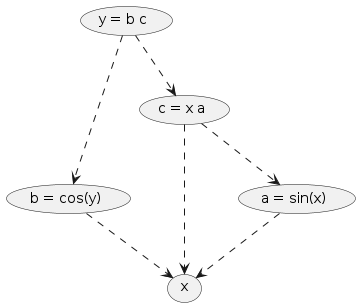
\includegraphics[width=0.5\linewidth]{differentiation/auto-diff-backward/example-nodes.png}
    \caption{後退型自動微分における計算グラフの例}
    \label{fig:differentiation_auto-diff_backward-nodes-example}
\end{figure}

\begin{algorithm}[tp]
    \caption{後退型自動微分における微分係数の計算}
    \label{alg:differentiation_auto-diff_backward-derivative-calculation}
    \begin{algorithmic}
        \Procedure{BackwardModeAutomaticDifferentiation}{グラフ, 微分の対象となるノード}
        \State $V, r = \text{ListRequiredNodes}(\text{グラフ, 微分の対象となるノード})$
        \Comment Algorithm \ref{alg:differentiation_auto-diff_backward-derivative-calculation-2}
        \ForAll{$V$ の要素 $v$}
        \State $d(v) \gets 0$ \Comment 微分係数
        \State $a(v) \gets 0$ \Comment 微分係数の加算を行った回数
        \EndFor
        \State $d(\text{微分の対象となるノード}) \gets 1$
        \State 空の処理待ちのキューを用意する.
        \State 処理待ちのキューに微分の対象となるノードを追加する.
        \While{処理待ちのキューに要素がある}
        \State 処理待ちのキューから要素を取り出し,$v$ とする.
        \ForAll{$v$ が参照しているノード $w$}
        \State $v$ を $w$ で偏微分した係数 $f$ を計算する.
        \State $d(w) \gets d(w) + f d(v)$
        \State $a(w) \gets a(w) + 1$
        \If{$a(w) = r(w)$}
        \State $w$ を処理待ちのキューに追加する.
        \EndIf
        \EndFor
        \EndWhile
        \EndProcedure
    \end{algorithmic}
\end{algorithm}
\begin{algorithm}[tp]
    \caption{後退型自動微分における微分係数の計算におけるサブルーチン ListRequiredNodes}
    \label{alg:differentiation_auto-diff_backward-derivative-calculation-2}
    \begin{algorithmic}
        \Procedure{ListRequiredNodes}{グラフ, 微分の対象となるノード}
        \State $V \gets \{\}$ \Comment 必要なノードの一覧
        \State $r(\text{微分の対象となるノード}) \gets 0$ \Comment ノードが参照されている回数
        \State 空の処理待ちのキューを用意する.
        \State 処理待ちのキューに微分の対象となるノードを追加する.
        \While{処理待ちのキューに要素がある}
        \State 処理待ちのキューから要素を取り出し,$v$ とする.
        \State $V \gets V + \{v\}$
        \ForAll{$v$ が参照しているノード $w$}
        \If{$r(w)$ が定義されている}
        \State $r(w) \gets r(w) + 1$
        \Else
        \State $r(w) \gets 1$
        \EndIf
        \If{$w$ が $V$ にない}
        \State $w$ を処理待ちのキューに追加する.
        \EndIf
        \EndFor
        \EndWhile
        \State \Return $V$, $r$
        \EndProcedure
    \end{algorithmic}
\end{algorithm}

後退型自動微分においては,
計算時とは逆順に微分係数の計算を行う必要がある.
そこで,
図 \ref{fig:differentiation_auto-diff_backward-nodes-example}
のような計算グラフと呼ばれるものを考える\cite{Kubota1998}.
図 \ref{fig:differentiation_auto-diff_backward-nodes-example}
の中で上の方にあるノードから順に微分係数の計算を進めていく方法としては,
例えば
Algorithm \ref{alg:differentiation_auto-diff_backward-derivative-calculation}
が考えられる
\footnote{文献 \cite{Kubota1998} には実装に使用できるレベルのアルゴリズムが見当たらなかったため,%
    トポロジカルソートをベースに考案した.}.


% !TEX root = ../main.tex
%

\part{正則化}

\chapter{導入}

この章では,正則化のアルゴリズムをまとめる.

未知のパラメータ $\bm{x}$ に合わせて変動するデータ $\bm{y} = A \bm{x}$ をもとに
パラメータ $\bm{x}$ を推定する問題は一般に逆問題と呼ばれる.
ここで,$\bm{x}$, $\bm{y}$ はそれぞれ何らかのノルム空間 $X$, $Y$ に存在するベクトルで,
$A$ は何らかの作用素とする.
例えば,録音した音源をもとに音が鳴っている場所を調べたい場合,
音が鳴っている場所が $\bm{x}$ であり,
録音した音源は $\bm{y}$ になる.

逆問題を解く単純な手法として,
ノルム $\|A \bm{x} - \bm{y}\|$ の最小化(最小二乗法)が挙げられるが,
作用素 $A$ の性質によっては,
$\bm{y}$ が少し変動するだけで最小二乗法による解 $\bm{x}$ が大きく変動してしまう場合があったり,
解が複数存在してしまう場合があったりする(ill-posed problem と呼ばれる).
そのような場合に,追加の情報をもとに唯一の安定な解を求められるようにする手法を正則化と呼ぶ.
ここでは,特に次のような式を最小化する正則化手法における数値解法をまとめる.

\begin{equation}
    \|A \bm{x} - \bm{y}\|^2 + \lambda R(\bm{x})
    \label{eq:regularization_intro_general-regularization}
\end{equation}

ここで,$\lambda \in [0, \infty)$ は正則化パラメータと呼ばれるパラメータで,
$R$ は $R : X \to [0, \infty)$ のような関数である.
この式を最小化する解 $\bm{x}_{\lambda}$ は正則化パラメータ $\lambda$ により変化する.
$\lambda = 0$ では正則化の効果がなくなり,
$\lambda$ を大きくすると正則化の効果が強くなる.
$\lambda$ を大きくしすぎると残差 $\|A \bm{x} - \bm{y}\|^2$ が大きくなり,
データ $\bm{y}$ から離れていってしまうため,
正則化パラメータ $\lambda$ を適切に調整することが必要となる.

\chapter{記号}

この章で使用する記号を以下に示す.

\begin{explainlist}
    $\setR$ & 実数の集合 \\
    $\setC$ & 複素数の集合 \\
    $\|\bm{x}\|$ & 一般のノルム \\
    $\|\bm{x}\|_2$ & ベクトル $\bm{x}$ の2-ノルム \\
    $A^*$ & 行列 $A$ のエルミート転置(随伴行列),または作用素 $A$ の随伴作用素 \\
    $A^{-*}$ & 行列 $A$ のエルミート転置の逆行列 \\
    $A^\dagger$ & 行列 $A$ の Moore-Penrose の一般化逆行列 \\
    $\diag(a_1, a_2, \ldots, a_n)$ & 対角要素に $a_1, a_2, \ldots, a_n$ を持つ対角行列 \\
    $\bm{a}_i$ & 行列 $A$ の $i$ 列目 \\
    $[A\bm{b}]_i$ & ベクトル $A\bm{b}$ の第 $i$ 要素
\end{explainlist}

% !TEX root = ../main.tex
%

\chapter{Tikhonov 正則化}

ここでは基本的な Tikhonov 正則化についてまとめる.
Tikhonov 正則化では,評価関数
\begin{equation}
    E_{\lambda}(x) \equiv \|A \bm{x} - \bm{y}\|_2^2 + \lambda \|\bm{x}\|_2^2
    \label{eq:regularization_tikhonov_objective}
\end{equation}
を最小化する.
ここで,
$\bm{x} \in \setC^n$,
$\bm{y} \in \setC^m$,
$A \in \setC^{m \times n}$
である.

\begin{theorem}\label{theorem:regularization_tikhonov_solution}
    $\lambda > 0$ の場合,
    評価関数 \eqref{eq:regularization_tikhonov_objective} が最小となるのは,
    $\bm{x} = (A^* A + \lambda I)^{-1} A^* \bm{y}$ の場合である.
\end{theorem}
\begin{proof}
    この場合,ノルムを展開することで,次のようになる.
    \begin{align}
        E_{\lambda}(x)
         & = \|A \bm{x} - \bm{y}\|_2^2 + \lambda \|\bm{x}\|_2^2
        \notag                                                                                              \\
         & = (A \bm{x} - \bm{y})^* (A \bm{x} - \bm{y}) + \lambda \bm{x}^* \bm{x}
        \notag                                                                                              \\
         & = \bm{x}^* (A^* A + \lambda I) \bm{x} - \bm{x}^* A^* \bm{y} - \bm{y}^* A \bm{x} + \|\bm{y}\|_2^2
    \end{align}
    ここで,
    $\lambda > 0$ の場合は
    $\bm{x} \neq \bm{0}$ において
    $\bm{x}^* (A^* A + \lambda I) \bm{x} = \|A \bm{x}\|_2^2 + \lambda \|\bm{x}\|_2^2 > 0$
    となることから,
    エルミート行列 $(A^* A + \lambda I)$ は正定値であり,
    正則となる.
    このことを用いると,さらに次のように展開できる.
    \begin{align}
        E_{\lambda}(x)
         & = \bm{x}^* (A^* A + \lambda I) \bm{x} - \bm{x}^* A^* \bm{y} - \bm{y}^* A \bm{x} + \|\bm{y}\|_2^2
        \notag                                                                                              \\
         & = \bm{x}^* (A^* A + \lambda I) \bm{x} - \bm{x}^* A^* \bm{y} - \bm{y}^* A \bm{x}
        + \bm{y}^* A (A^* A + \lambda I)^{-1} A^* \bm{y}
        - \bm{y}^* A (A^* A + \lambda I)^{-1} A^* \bm{y}
        + \|\bm{y}\|_2^2
        \notag                                                                                              \\
         & = (\bm{x} - (A^* A + \lambda I)^{-1} A^* \bm{y})^*
        (A^* A + \lambda I)
        (\bm{x} - (A^* A + \lambda I)^{-1} A^* \bm{y})
        - \bm{y}^* A (A^* A + \lambda I)^{-1} A^* \bm{y}
        + \|\bm{y}\|_2^2
    \end{align}
    エルミート行列 $(A^* A + \lambda I)$ が正定値であることから,
    この式が最小となるのは
    $(\bm{x} - (A^* A + \lambda I)^{-1} A^* \bm{y})$
    が零ベクトルとなる場合,
    つまり,
    $\bm{x} = (A^* A + \lambda I)^{-1} A^* \bm{y}$
    の場合である.
\end{proof}

ここで,$\lambda = 0$ でも,行列 $A$ のランクが $n$ の場合は $A^*A$ が正定値になるため同様に解が求まる.

\section{特異値分解による解法}

行列 $A$ を次のように特異値分解する.

\begin{equation}
    A = U
    \begin{pmatrix}
        \Sigma & O \\
        O      & O
    \end{pmatrix}
    V^*
\end{equation}

ここで,$U \in \setC^{m \times m}$ と $V \in \setC^{n \times n}$ はユニタリ行列で,
$\Sigma \in \setR^{r \times r}$ は正の実数による対角行列である.
ただし,ランク $r$ は $m$ または $n$ に等しくても良い.

この分解を用いると,
定理 \ref{theorem:regularization_tikhonov_solution} の解は次のように変形できる.

\begin{align}
    x_{\lambda}
     & \equiv (A^* A + \lambda I)^{-1} A^* \bm{y}
    \notag                                        \\
     & = \left(V
    \begin{pmatrix}
        \Sigma & O \\
        O      & O
    \end{pmatrix}
    U^* U
    \begin{pmatrix}
        \Sigma & O \\
        O      & O
    \end{pmatrix}
    V^* + \lambda I \right)^{-1}
    V
    \begin{pmatrix}
        \Sigma & O \\
        O      & O
    \end{pmatrix}
    U^* \bm{y}
    \notag                                        \\
     & = \left(V
    \begin{pmatrix}
        \Sigma^2 & O \\
        O        & O
    \end{pmatrix}
    V^* + \lambda V V^* \right)^{-1}
    V
    \begin{pmatrix}
        \Sigma & O \\
        O      & O
    \end{pmatrix}
    U^* \bm{y}
    \notag                                        \\
     & = \left(V
    \begin{pmatrix}
        \Sigma^2 + \lambda I & O         \\
        O                    & \lambda I
    \end{pmatrix}
    V^* \right)^{-1}
    V
    \begin{pmatrix}
        \Sigma & O \\
        O      & O
    \end{pmatrix}
    U^* \bm{y}
    \notag                                        \\
     & = V
    \begin{pmatrix}
        (\Sigma^2 + \lambda I)^{-1} & O              \\
        O                           & \lambda^{-1} I
    \end{pmatrix}
    V^*
    V
    \begin{pmatrix}
        \Sigma & O \\
        O      & O
    \end{pmatrix}
    U^* \bm{y}
    \notag                                        \\
     & = V
    \begin{pmatrix}
        (\Sigma^2 + \lambda I)^{-1} \Sigma & O \\
        O                                  & O
    \end{pmatrix}
    U^* \bm{y}
\end{align}

さらに,
$U = (\bm{u}_1, \bm{u}_2, \ldots, \bm{u}_m)$,
$V = (\bm{v}_1, \bm{v}_2, \ldots, \bm{v}_n)$,
$\Sigma = \diag(\sigma_1, \sigma_2, \ldots, \sigma_r)$
とすると,次のように表記できる.

\begin{align}
    x_{\lambda}
     & = \sum_{i = 1}^{r} \frac{\sigma_i}{\sigma_i^2 + \lambda} (\bm{u}_i^* \bm{y}) \bm{v}_i
\end{align}

特異値分解を一回行い
$\bm{u}_i^* \bm{y}$
を計算しておけば,
ある正則化パラメータ $\lambda$ に対する解 $\bm{x}_{\lambda}$ は単純な線形和で求めることができる.

また,
$U_1 \equiv (\bm{u}_1, \bm{u}_2, \ldots, \bm{u}_r)$,
$U_2 \equiv (\bm{u}_{r+1}, \bm{u}_{r+2}, \ldots, \bm{u}_m)$
と定義した場合,$U$ がユニタリ行列であることから
$U_1^* U_1 = I$,
$U_1^* U_2 = O$,
$U_2^* U_1 = O$,
$U_2^* U_2 = I$,
$U_1 U_1^* + U_2 U_2^* = I$
が成り立つことを利用すると,
正則化パラメータを評価する際にしばしば利用される評価関数内のノルムは次のように計算できる
\footnote{行列 $U$ のうち $U_1$ の部分だけを求めた方が計算コストを抑えられるため,%
    $U_2$ はなるべく使用しない計算式を求めている.}.

\begin{align}
    \|A \bm{x}_{\lambda} - \bm{y}\|_2^2
     & = \left\| U
    \begin{pmatrix}
        \Sigma & O \\
        O      & O
    \end{pmatrix}
    V^* V
    \begin{pmatrix}
        (\Sigma^2 + \lambda I)^{-1} \Sigma & O \\
        O                                  & O
    \end{pmatrix}
    U^* \bm{y} - \bm{y} \right\|_2^2
    \notag                                                                                        \\
     & = \left\|
    \begin{pmatrix}
        U_1 & U_2
    \end{pmatrix}
    \begin{pmatrix}
        \Sigma (\Sigma^2 + \lambda I)^{-1} \Sigma & O \\
        O                                         & O
    \end{pmatrix}
    \begin{pmatrix}
        U_1^* \\ U_2^*
    \end{pmatrix}
    \bm{y} - \bm{y} \right\|_2^2
    \notag                                                                                        \\
     & = \left\| U_1 \Sigma (\Sigma^2 + \lambda I)^{-1} \Sigma U_1^* \bm{y} - \bm{y} \right\|_2^2
    \notag                                                                                        \\
     & = \left\| U_1 \Sigma (\Sigma^2 + \lambda I)^{-1} \Sigma U_1^* \bm{y}
    - U_1 U_1^* \bm{y} - U_2 U_2^* \bm{y} \right\|_2^2
    \notag                                                                                        \\
     & = \left\| U_1 (\Sigma (\Sigma^2 + \lambda I)^{-1} \Sigma - I) U_1^* \bm{y}
    - U_2 U_2^* \bm{y} \right\|_2^2
    \notag                                                                                        \\
     & = \left\| U_1 (\Sigma (\Sigma^2 + \lambda I)^{-1} \Sigma - I) U_1^* \bm{y} \right\|_2^2
    + \left\| U_2 U_2^* \bm{y} \right\|_2^2
    \notag                                                                                        \\
     & = \left\| (\Sigma (\Sigma^2 + \lambda I)^{-1} \Sigma - I) U_1^* \bm{y} \right\|_2^2
    + \left\| U_2 U_2^* \bm{y} \right\|_2^2
    \notag                                                                                        \\
     & = \sum_{i = 1}^r \left(\frac{\lambda}{\sigma_i^2 + \lambda}\right)^2 (\bm{u}_i^* \bm{y})^2
    + \left\| (I - U_1 U_1^*) \bm{y} \right\|_2^2
\end{align}

\begin{align}
    \|\bm{x}_{\lambda}\|_2^2
     & = \left\| V
    \begin{pmatrix}
        (\Sigma^2 + \lambda I)^{-1} \Sigma & O \\
        O                                  & O
    \end{pmatrix}
    U^* \bm{y} \right\|_2^2
    \notag                                                                                          \\
     & = \left\|
    \begin{pmatrix}
        (\Sigma^2 + \lambda I)^{-1} \Sigma & O \\
        O                                  & O
    \end{pmatrix}
    U^* \bm{y} \right\|_2^2
    \notag                                                                                          \\
     & = \sum_{i = 1}^r \left(\frac{\sigma_i}{\sigma_i^2 + \lambda}\right)^2  (\bm{u}_i^* \bm{y})^2
\end{align}

どちらも正則化パラメータごとに異なる部分は $O(r)$ オーダーで計算できる.

特異値分解による Tikhonov 正則化では,
正則化パラメータを変更した際の再計算が容易なため,
多数の正則化パラメータを試したい場合に便利である.

% !TEX root = ../main.tex
%

\chapter{一般化 Tikhonov 正則化}

前章の Tikhonov 正則化では,
正則化項が $\|\bm{x}\|_2^2$ となっていたが,
正則化項として係数行列を追加した $\|L\bm{x}\|_2^2$ を用いることも考えられる.
例えば,変数 $\bm{x}$ の隣り合う要素の差をとるように係数行列 $L$ を決めることにより,
解が滑らかになるような正則化を行うことができる.
このような一般化した Tikhonov 正則化では,評価関数
\begin{equation}
    E_{\lambda}(\bm{x}) \equiv \|A \bm{x} - \bm{y}\|_2^2 + \lambda \|L \bm{x}\|_2^2
    \label{eq:regularization_gen-tikhonov_objective}
\end{equation}
を最小化する.
ここで,
$\bm{x} \in \setC^n$,
$\bm{y} \in \setC^m$,
$A \in \setC^{m \times n}$,
$L \in \setC^{p \times n}$
である.

ここで,正則化項の変更により注意することがある.
Tikhonov 正則化では,$\lambda > 0$ であれば解が唯一となっていた
(定理 \ref{theorem:regularization_tikhonov_solution}).
しかし,一般化 Tikhonov 正則化においては,
$\lambda > 0$ であるからといって解が唯一になるとは限らない.

\begin{theorem}
    $A$ と $L$ の核空間の共通部分が $\bm{0}$ 以外の要素を持つ場合,
    $\lambda > 0$ であったとしても
    評価関数 \eqref{eq:regularization_gen-tikhonov_objective} が最小となる $\bm{x}$ が
    唯一に定まらない.
\end{theorem}
\begin{proof}
    評価関数 \eqref{eq:regularization_gen-tikhonov_objective} が最小となる
    $\bm{x}$ の 1 つを $\bar{\bm{x}}$ とする.
    また,$A$ と $L$ の核空間の共通部分が $\bm{0}$ 以外に持つ要素の 1 つを $\bm{x}_0$ とする.
    このとき,
    \begin{align}
        E_{\lambda}(\bar{\bm{x}} + \bm{x}_0)
         & = \|A (\bar{\bm{x}} + \bm{x}_0) - \bm{y}\|_2^2 + \lambda \|L (\bar{\bm{x}} + \bm{x}_0)\|_2^2
        \notag                                                                                          \\
         & = \|A \bar{\bm{x}} - \bm{y}\|_2^2 + \lambda \|L \bar{\bm{x}}\|_2^2
        \notag                                                                                          \\
         & = E(\bar{\bm{x}})
    \end{align}
    となる.
    よって,評価関数 $E(\bm{x})$ が最小となる $\bm{x}$ は唯一に定まらない.
\end{proof}

一方,$A$ と $L$ の核空間の共通部分が $\bm{0}$ のみであれば
$\lambda > 0$ のときに解が唯一となる.

\begin{theorem}\label{theorem:regularization_gen-tikhonov_solution}
    $A$ と $L$ の核空間の共通部分が $\bm{0}$ のみでかつ,
    $\lambda > 0$ の場合,
    評価関数 \eqref{eq:regularization_gen-tikhonov_objective} が最小となるのは,
    $\bm{x} = (A^* A + \lambda L^* L)^{-1} A^* \bm{y}$ の場合である.
\end{theorem}
\begin{proof}
    この場合,ノルムを展開することで,次のようになる.
    \begin{align}
        E_{\lambda}(\bm{x})
         & = \|A \bm{x} - \bm{y}\|_2^2 + \lambda \|L \bm{x}\|_2^2
        \notag                                                                                                  \\
         & = (A \bm{x} - \bm{y})^* (A \bm{x} - \bm{y}) + \lambda \bm{x}^* L^* L \bm{x}
        \notag                                                                                                  \\
         & = \bm{x}^* (A^* A + \lambda L^* L) \bm{x} - \bm{x}^* A^* \bm{y} - \bm{y}^* A \bm{x} + \|\bm{y}\|_2^2
    \end{align}
    ここで,
    $A$ と $L$ の核空間の共通部分が $\bm{0}$ のみでかつ
    $\lambda > 0$ の場合は
    $\bm{x} \neq \bm{0}$ において
    $\bm{x}^* (A^* A + \lambda L^* L) \bm{x} = \|A \bm{x}\|_2^2 + \lambda \|L \bm{x}\|_2^2 > 0$
    となることから,
    エルミート行列 $(A^* A + \lambda I)$ は正定値であり,
    正則となる.
    このことを用いると,さらに次のように展開できる.
    \begin{align}
        E_{\lambda}(\bm{x})
         & = \bm{x}^* (A^* A + \lambda L^* L) \bm{x} - \bm{x}^* A^* \bm{y} - \bm{y}^* A \bm{x} + \|\bm{y}\|_2^2
        \notag                                                                                                  \\
         & = \bm{x}^* (A^* A + \lambda L^* L) \bm{x} - \bm{x}^* A^* \bm{y} - \bm{y}^* A \bm{x}
        + \bm{y}^* A (A^* A + \lambda L^* L)^{-1} A^* \bm{y}
        - \bm{y}^* A (A^* A + \lambda L^* L)^{-1} A^* \bm{y}
        + \|\bm{y}\|_2^2
        \notag                                                                                                  \\
         & = (\bm{x} - (A^* A + \lambda L^* L)^{-1} A^* \bm{y})^*
        (A^* A + \lambda L^* L)
        (\bm{x} - (A^* A + \lambda L^* L)^{-1} A^* \bm{y})
        - \bm{y}^* A (A^* A + \lambda L^* L)^{-1} A^* \bm{y}
        + \|\bm{y}\|_2^2
    \end{align}
    エルミート行列 $(A^* A + \lambda L^* L)$ が正定値であることから,
    この式が最小となるのは
    $(\bm{x} - (A^* A + \lambda L^* L)^{-1} A^* \bm{y})$
    が零ベクトルとなる場合,
    つまり,
    $\bm{x} = (A^* A + \lambda L^* L)^{-1} A^* \bm{y}$
    の場合である.
\end{proof}

\section{一般化 Tikhonov 正則化}

$m \ge n \ge p$ の場合は
次のように表される一般化特異値分解を行うことができる \cite{Hansen1998}.

\begin{align}
    A       & =U
    \begin{pmatrix}
        \Sigma & O \\
        O      & I
    \end{pmatrix}
    W^{-1}, &
    L       & =V
    \begin{pmatrix}
        M & O
    \end{pmatrix}
    W^{-1}
\end{align}

ここで,
$U \in \setC^{m \times n}$,
$V \in \setC^{p \times p}$
はユニタリ行列で,
$W \in \setC^{n \times n}$
は正則行列とし,
$\Sigma = \diag(\sigma_1, \sigma_2, \ldots, \sigma_p)$,
$M = \diag(\mu_1, \mu_2, \ldots, \mu_p)$
は対角行列である.
$\sigma_i$ と $\mu_i$ については
$0 \le \sigma_1 \le \sigma_2 \le \ldots \le \sigma_p \le 1$,
$1 \ge \mu_1 \ge \mu_2 \ge \ldots \ge \mu_p > 0$,
$\sigma_i^2 + \mu_i^2 = 1$
を満たすものとし,
$\gamma_i = \sigma_i / \mu_i$
を一般化特異値と呼ぶ.
これを用いると,
次のように評価関数 \eqref{eq:regularization_gen-tikhonov_objective} を最小化する
$\bm{x}$ を表せる\cite{Hansen1998}.

\begin{equation}
    \bm{x}_\lambda =
    \sum_{i=1}^{p} \frac{\gamma_i / \mu_i}{\gamma_i^2+\lambda}
    (\bm{u}^*\bm{y}) \bm{w}_i
    +\sum_{i=p+1}^n (\bm{u}_i^*\bm{y}) \bm{w}_i
\end{equation}

$L=I$ のときこの式が Tikhonov 正則化の場合の
式 \eqref{eq:regularization_tikhonov_solution-by-svd} に一致することは
簡単に確かめられる.

% !TEX root = ../main.tex
%

\chapter{L-curve}

ここでは正則化パラメータを決める手法の1つである
L-curve法について説明する.

\begin{figure}[tp]\centering
    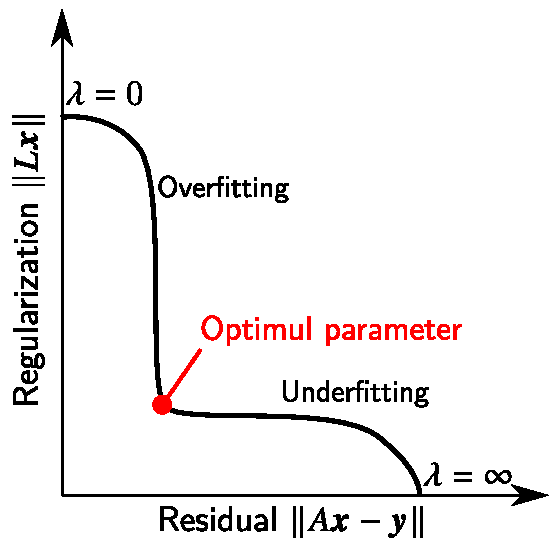
\includegraphics{./regularization/L-curve.pdf}
    \caption{L-curve の概形}
    \label{fig:regularization_l-curve_l-curve}
\end{figure}

正則化の式 \eqref{eq:regularization_intro_general-regularization} を最小化する
$\bm{x}$ を $\bm{x}_\lambda$ として,
横軸を残差 $\|A\bm{x}_\lambda-\bm{y}\|$,
縦軸を正則化項 $R(\bm{x}_\lambda)$ とし,
正則化パラメータ $\lambda$ を変えたときの
プロットを L-curve と呼ぶ.
L-curve は一般に図 \ref{fig:regularization_l-curve_l-curve} のような L の字を
描いている場合が多い.
単純にノルムをプロットするよりも
両対数グラフにプロットする方が
後述する曲線の特徴をはっきりさせられる他,
スケールの違いによる影響を
抑えられるなどのメリットもあるという
\cite{Hansen1998}.

図 \ref{fig:regularization_l-curve_l-curve} のように L-curve が得られた場合,
L の字の曲がり角にあたる赤い点の部分から左上の方では
残差がほとんど減らずに正則化項が増加しており,
右下の方では正則化項がほとんど減らずに残差が増えているため,
両方のバランスが取れている L の字の曲がり角を取るのが良いと考えられる.
そこで,L-curve の曲がり角を数値的に求める手法について考える.

ここでは,文献 \cite{Hansen1998} に従い次の関数の組を考える.
\begin{equation}
    (\xi(\lambda), \eta(\lambda))
    =(\log\|A \bm{x}_\lambda - \bm{y}\|, \log{R(\bm{x})})
\end{equation}
L-curve の曲がり角は曲線 $(\xi(\lambda), \eta(\lambda))$ の
曲率が最も大きい部分と考えられるため,曲率
\begin{equation}
    \kappa(\lambda) =
    \frac{\xi'\eta'' - \xi''\eta'}
    {\left( (\xi')^2 + (\eta')^2 \right)^{3/2}}
    \label{eq:regularization_l-curve_curvature}
\end{equation}
を求め,それを最大化する.
曲率が何らかの手法で求まれば,
1 変数の最適化については
\ref{chap:opt_one-dim-section-search} 章で説明しているため,
ここでは曲率の計算法について考える.

\section{Tikhonov 正則化の場合}

Tikhonov 正則化(\ref{chap:regularization_tikhonov} 章)の場合,
式 \eqref{eq:regularization_l-curve_curvature} にある各種微分を
陽的に表すことができる
\cite{Hansen1992,Mueller2012}.

\begin{align}
    \frac{d}{d\lambda} \|A \bm{x}_\lambda - \bm{y}\|_2^2
     & = \sum_{i=1}^r \frac{2 \lambda \sigma_i^2}{(\sigma_i^2 + \lambda)^3}
    \left(\bm{u}_i^* \bm{y}\right)^2
    \\
    \frac{d}{d\lambda} \|\bm{x}_\lambda\|_2^2
     & = \sum_{i=1}^r \frac{-2 \sigma_i^2}{(\sigma_i^2 + \lambda)^3}
    \left(\bm{u}_i^* \bm{y}\right)^2
    \\
    \frac{d^2}{d\lambda^2} \|A \bm{x}_\lambda - \bm{y}\|_2^2
     & = \sum_{i=1}^r \frac{2 \sigma_i^4 - 4 \lambda \sigma_i^2}
    {(\sigma_i^2 + \lambda)^4}
    \left(\bm{u}_i^* \bm{y}\right)^2
    \\
    \frac{d^2}{d\lambda^2} \|\bm{x}_\lambda\|_2^2
     & = \sum_{i=1}^r \frac{6 \sigma_i^2}{(\sigma_i^2 + \lambda)^4}
    \left(\bm{u}_i^* \bm{y}\right)^2
\end{align}

これらは式
\eqref{eq:regularization_tikhonov_residual-by-svd},
\eqref{eq:regularization_tikhonov_regularization-term-by-svd}
から求めることができる.


% !TEX root = ../main.tex
%

\part{補間}

\chapter{導入}

この部では,補間の手法をまとめる.
補間では,
サンプル点 $(\bm{r}_i, y_i) \in X \times \setC$ ($i = 1, 2, \ldots, m$) について
$f(\bm{r}_i) = y_i$
となるような関数 $f$ を算出する.
データがノイズを含んでいる場合は
正則化(\ref{part:regularization} 部)を利用して
$f(\bm{r}_i) \approx y_i$
となるような関数 $f$ を求める場合もある.

% !TEX root = ../main.tex
%

\chapter{カーネル法}

\index{かーねるほう@カーネル法}
本章では,カーネルを用いて補間を行うカーネル法についてまとめる.

関数 $f : X \to \setC$ を
サンプル点 $(\bm{r}_i, y_i) \in X \times \setC$ ($i = 1, 2, \ldots, m$) から補間することを考える.
カーネルを用いた補間では,カーネル $K : X \times X \to \setC$ を用いて
\begin{equation}
    f(\bm{r}) = \sum_{i=1}^m c_i K(\bm{r}, \bm{r}_i)
\end{equation}
のようにおき,$y_i = f(\bm{r}_i)$ となるように係数 $c_i$ を決める
\cite{Fukumizu2010}.

\section{Tikhonov 正則化による導出}\label{sec:interp_kernel_tikhonov}

まず,カーネルによる補間の導出を行う.

関数 $f$ はある正規直交基底の存在する関数空間 $\mathcal{H}$
\footnote{正確には,関数空間 $\mathcal{H}$ には%
    再生核ヒルベルト空間 (reproducing kernel Hilbert space, RKHS)%
    と呼ばれるものを用いる.}
に属するものとし,
その関数空間 $\mathcal{H}$ には正規直交基底となる
関数 $\alpha_1(\bm{r}), \alpha_2(\bm{r}), \ldots, \alpha_N(\bm{r})$ が存在するものとする
\footnote{この導出では $N$ が有限であるとする.}.
それらの基底を用いて関数 $f$ を次のようにおく.
\begin{equation}
    f(\bm{r}) = \sum_{i = 1}^{N} x_i \alpha_i(\bm{r})
\end{equation}
ここで,
$A_{ij} = \alpha_j(\bm{r}_i)$ となる行列 $A \in \setC^{m \times N}$ を考えると,
最小二乗法の評価関数は
\begin{equation}
    \|A \bm{x} - \bm{y}\|_2
\end{equation}
となる.

これに Tikhonov 正則化(\ref{chap:regularization_tikhonov} 章)を適用する.
関数空間 $\mathcal{H}$ のノルムを $\|\cdot\|_{\mathcal{H}}$ とすると,
$\alpha_i$ が $\mathcal{H}$ の正規直交基底であることから,
\begin{align}
    \|f\|_{\mathcal{H}}^2
     & = \sum_{i = 1}^{N} |x_i|^2 \notag \\
     & = \|\bm{x}\|_2^2
\end{align}
となる.
よって,Tikhonov 正則化の評価関数は
式 \eqref{eq:regularization_tikhonov_objective} のように書ける.

式 \eqref{eq:regularization_tikhonov_exchange-mat} より最適解は
\begin{align}
    \bm{x} & = A^* (AA^* + \lambda I)^{-1} \bm{y}
\end{align}
となる.
ここで,行列 $AA^*$ の $(i, j)$ 要素は
\begin{equation}
    [AA^*]_{ij} = \sum_{k = 1}^{N} \alpha_k(\bm{r}_i) \overline{\alpha_k(\bm{r}_j)}
\end{equation}
となる.それをもとに次のように関数 $K : X \times X \to \setC$ を定義する.
\begin{equation}
    K(\bm{r}, \bm{r}') = \sum_{k = 1}^{N} \alpha_k(\bm{r}) \overline{\alpha_k(\bm{r}')}
\end{equation}
この関数がカーネルである.
また,行列 $K_m \in \setC^{m \times m}$ を
$K_m = AA^*$ のようにおく.
なお,この行列は半正定値エルミート行列である.

ここで,変数 $\bm{c} \in \setC^m$ を
\begin{equation}
    \bm{c} = (K_m + \lambda I)^{-1} \bm{y}
    \label{eq:interp_kernel_tikhonov_coeff_c}
\end{equation}
のようにおく.
このとき,$\bm{x} = A^* \bm{c}$ だから,
\begin{align}
    f(\bm{r})
     & = \sum_{i = 1}^{N} x_i \alpha_i(\bm{r}) \notag                                                \\
     & = \sum_{i = 1}^{N} \sum_{j = 1}^{m} \overline{A_{ji}} c_j \alpha_i(\bm{r}) \notag             \\
     & = \sum_{i = 1}^{N} \sum_{j = 1}^{m} \overline{\alpha_i(\bm{r}_j)} c_j \alpha_i(\bm{r}) \notag \\
     & = \sum_{j = 1}^{m} c_j K(\bm{r}, \bm{r}_j)
\end{align}
となる.

関数 $f$ を正規直交基底で表していたことから,
カーネル法は関数空間 $\mathcal{H}$ 全体の中で Tikhonov 正則化の評価関数
\begin{equation}
    \sum_{i=1}^m \left|y_i - f(\bm{r}_i)\right|^2
    + \|f\|_{\mathcal{H}}^2
\end{equation}
を最小化したものを求められるということが分かる.
また,ここでは導出において関数空間 $\mathcal{H}$ の次元を表す $N$ が有限であることを前提としていたが,
導出されたカーネル法で用いる行列は $m \times m$ の正方行列であるため,
$N \to \infty$ の場合にも適用できる.

\section{Gaussian Process}\label{sec:regularization_kernel_gaussian-process}

カーネルによる補間は,
\index{Gaussian Process}
Gaussian Process と呼ばれる確率分布から導くこともできる
\cite{Brochu2010}.
ただし,データとカーネル関数の値は実数とする.

平均 $\mu(\bm{r})$,分散 $K(\bm{r}, \bm{r}')$ の Gaussian Process に従う関数 $f$ は,
関数値のベクトル $(f(\bm{r}_1), f(\bm{r}_2), \ldots, f(\bm{r}_m))$ が
正規分布 $\mathcal{N}(\bm{\mu}_m, K_m)$ に従う.
ここで,
$\bm{\mu}_m$ は $[\bm{\mu}_m]_i = \mu(\bm{r}_i)$ なるベクトルであり,
$K_m$ は $[K_m]_{ij} = K(\bm{r}_i, \bm{r}_j)$ なる行列である.
Gaussian Process は関数における正規分布のようなものである.

関数 $f$ が平均 $0$,分散 $\tau K(\bm{r}, \bm{r}')$ の Gaussian Process に従っており,
関数 $f$ に対するノイズ入りのサンプルが $y_i = f(\bm{r}_i) + \epsilon_i$ のように得られているとする.
ただし,$\epsilon_i$ は独立に正規分布 $\mathcal{N}(0, \sigma^2)$ に従うものとする.
また,$\tau > 0$ は分散の大きさを示すパラメータである.
このとき,ベクトル $(y_1, y_2, \ldots, y_m, f(\bm{r}))$ は
次のような正規分布に従う.
\begin{equation}
    \mathcal{N}\left(\bm{0},
    \begin{pmatrix}
        \tau K_m + \sigma^2 I & \tau \bm{k}(\bm{r})    \\
        \tau \bm{k}(\bm{r})^T & \tau K(\bm{r}, \bm{r})
    \end{pmatrix}
    \right)
\end{equation}
このとき,確率密度関数 $p(y_1, y_2, \ldots, y_m, f(\bm{r}))$ は次のように書ける.
\begin{equation}
    p(y_1, y_2, \ldots, y_m, f(\bm{r}))
    = \frac{1}{\sqrt{(2\pi)^{m+1} \det{
                \begin{pmatrix}
                    \tau K_m + \sigma^2 I & \tau \bm{k}(\bm{r})    \\
                    \tau \bm{k}(\bm{r})^T & \tau K(\bm{r}, \bm{r})
                \end{pmatrix}
            }}}
    \exp\left(-\frac{1}{2}
    \begin{pmatrix}
        \bm{y} \\ f(\bm{r})
    \end{pmatrix}^T
    \begin{pmatrix}
        \tau K_m + \sigma^2 I & \tau \bm{k}(\bm{r})    \\
        \tau \bm{k}(\bm{r})^T & \tau K(\bm{r}, \bm{r})
    \end{pmatrix}^{-1}
    \begin{pmatrix}
        \bm{y} \\ f(\bm{r})
    \end{pmatrix}
    \right)
\end{equation}

ここで,
\begin{align}
    \sigma_K^2(\bm{r})
     & \equiv \tau K(\bm{r}, \bm{r})
    - \tau \bm{k}(\bm{r})^T (\tau K_m + \sigma^2 I)^{-1} \tau \bm{k}(\bm{r}) \\
     & = \tau K(\bm{r}, \bm{r})
    - \tau \bm{k}(\bm{r})^T (K_m + \sigma^2 I)^{-1} \bm{k}(\bm{r})
\end{align}
とおくと,
\begin{align}
    \det{
        \begin{pmatrix}
            \tau K_m + \sigma^2 I & \tau \bm{k}(\bm{r})    \\
            \tau \bm{k}(\bm{r})^T & \tau K(\bm{r}, \bm{r})
        \end{pmatrix}
    }
     & = \sigma_K^2(\bm{r}) \det(\tau K_m + \sigma^2 I)
\end{align}
となる.
また,
\begin{align}
     & \hphantom{=}
    \begin{pmatrix}
        \tau K_m + \sigma^2 I & \tau \bm{k}(\bm{r})    \\
        \tau \bm{k}(\bm{r})^T & \tau K(\bm{r}, \bm{r})
    \end{pmatrix}^{-1}
    \notag          \\
     & =
    \begin{pmatrix}
        (\tau K_m + \sigma^2 I)^{-1}
        + (\tau K_m + \sigma^2 I)^{-1} \tau \bm{k}(\bm{r}) \sigma_K^2(\bm{r})^{-1} \tau \bm{k}(\bm{r})^T (\tau K_m + \sigma^2 I)^{-1}
         &
        - (\tau K_m + \sigma^2 I)^{-1} \tau \bm{k}(\bm{r}) \sigma_K^2(\bm{r})^{-1}
        \\
        - \sigma_K^2(\bm{r})^{-1} \tau \bm{k}(\bm{r})^T (\tau K_m + \sigma^2 I)^{-1}
         &
        \sigma_K^2(\bm{r})^{-1}
    \end{pmatrix}
\end{align}
であり,
\begin{align}
     & \hphantom{=}
    \begin{pmatrix}
        \bm{y} \\ f(\bm{r})
    \end{pmatrix}^T
    \begin{pmatrix}
        \tau K_m + \sigma^2 I & \tau \bm{k}(\bm{r})    \\
        \tau \bm{k}(\bm{r})^T & \tau K(\bm{r}, \bm{r})
    \end{pmatrix}^{-1}
    \begin{pmatrix}
        \bm{y} \\ f(\bm{r})
    \end{pmatrix}
    \notag                                            \\
     & = \bm{y}^T (\tau K_m + \sigma^2 I)^{-1} \bm{y}
    + \bm{y}^T (\tau K_m + \sigma^2 I)^{-1} \tau \bm{k}(\bm{r}) \sigma_K^2(\bm{r})^{-1} \tau \bm{k}(\bm{r})^T (\tau K_m + \sigma^2 I)^{-1} \bm{y}
    \notag                                            \\ & \hspace{2em}
    - f(\bm{r}) \sigma_K^2(\bm{r})^{-1} \tau \bm{k}(\bm{r})^T (\tau K_m + \sigma^2 I)^{-1} \bm{y}
    - \bm{y}^T (\tau K_m + \sigma^2 I)^{-1} \tau \bm{k}(\bm{r}) \sigma_K^2(\bm{r})^{-1} f(\bm{r})
    \notag                                            \\ & \hspace{2em}
    + f(\bm{r}) \sigma_K^2(\bm{r})^{-1} f(\bm{r})
    \notag                                            \\
     & = \bm{y}^T (\tau K_m + \sigma^2 I)^{-1} \bm{y}
    + \sigma_K^2(\bm{r})^{-1} \left(f(\bm{r}) - \tau \bm{k}(\bm{r})^T (\tau K_m + \sigma^2 I)^{-1} \bm{y}\right)^2
\end{align}
となる.
よって,確率密度関数は次のように分割できる.
\begin{align}
    p(y_1, y_2, \ldots, y_m, f(\bm{r}))
     & = p_{\bm{y}}(\bm{y}) p_f(f(\bm{r}))
    \\
    p_{\bm{y}}(\bm{y})
     & = \frac{1}{\sqrt{(2\pi)^{m} \det(\tau K_m + \sigma^2 I)}}
    \exp\left(-\frac{1}{2} \bm{y}^T (\tau K_m + \sigma^2 I)^{-1} \bm{y} \right)
    \\
    p_f(f(\bm{r}))
     & = \frac{1}{\sqrt{(2\pi)^{m} \sigma_K^2(\bm{r})}}
    \exp\left(-\frac{1}{2} \sigma_K^2(\bm{r})^{-1} \left(f(\bm{r}) - \mu_K(\bm{r})\right)^2\right)
    \\
    \mu_K(\bm{r})
     & = \tau \bm{k}(\bm{r})^T (\tau K_m + \sigma^2 I)^{-1} \bm{y}
\end{align}
分割したあとの
$p_{\bm{y}}$ は $\bm{y}$ に関する正規分布 $\mathcal{N}(\bm{0}, \tau K_m + \sigma^2 I)$ であり,
$p_f$ は $f(\bm{r})$ に関する正規分布 $\mathcal{N}(\mu_K(\bm{r}), \sigma_K^2(\bm{r}))$ である.
$\lambda = \sigma^2 / \tau$ とおくと,
\begin{align}
    \mu_K(\bm{r})
     & = \tau \bm{k}(\bm{r})^T (\tau K_m + \sigma^2 I)^{-1} \bm{y}
    \notag                                                                               \\
     & = \bm{k}(\bm{r})^T (K_m + \lambda I)^{-1} \bm{y}
    \notag                                                                               \\
     & = \sum_{i = 1}^m K(\bm{r}, \bm{r}_i) \left[(K_m + \lambda I)^{-1} \bm{y}\right]_i
\end{align}
のように前節と同様の公式が得られる.

Gaussian Process を用いた表現では分散 $\sigma_K^2(\bm{r})$ も得られるため,
補間された関数のどの部分に誤差が多い可能性が高いか評価するのにも役立つ.
また,パラメータ推定において確率の最大化を行うといった応用もある
(\ref{sec:regularization_kernel_param-est} 節).

\section{RBF 補間}\label{sec:interp_kernel_rbf}

\index{RBFほかん@RBF 補間}
\index{Radial Basis Function}
カーネル $K(\bm{r}, \bm{r}')$ の値が距離 $\|\bm{r} - \bm{r}'\|_2$ に依存する場合,
そのもとになる関数は Radial Basis Function (RBF) と呼ばれる.
RBF $\phi : [0, \infty) \to \setR$ によるカーネルは
\begin{equation}
    K(\bm{r}, \bm{r}') = \phi\left(\frac{\|\bm{r} - \bm{r}'\|_2}{c}\right)
    \label{eq:regularization_kernel_kernel-of-rbf}
\end{equation}
のように書ける.
RBF としては表
\ref{table:interp_kernel_example-rbfs}
のようなものが挙げられる
\cite{Brochu2010,Fornberg2015}.

\begin{table}[bp]
    \caption{RBF の例 \cite{Brochu2010,Fornberg2015}}
    \label{table:interp_kernel_example-rbfs}
    \centering
    \begin{tabular}{ll}
        名称                      & 関数                         \\
        \hline
        Gaussian                & $e^{-r^2}$                 \\
        Multi-quadric           & $\sqrt{1 + r^2}$           \\
        Inverse Multi-quadric   & $1/\sqrt{1 + r^2}$         \\
        Inverse Quadric         & $1 / (1 + r^2)$            \\
        Bessel ($d=1,2,\ldots$) & $J_{d/2-1}(r) / r^{d/2-1}$
    \end{tabular}
\end{table}

\section{パラメータ推定}\label{sec:regularization_kernel_param-est}

式 \eqref{eq:regularization_kernel_kernel-of-rbf} の定数 $c$ のように
カーネルがパラメータを持っている場合がある.
そのようなパラメータの推定を
\cite[Remark 3 (Connection to spatial statistics)]{Scheuerer2011}
に沿った
\index{maximum likelihood estimation}
maximum likelihood estimation (MLE)
により考える.

Gaussian Process (\ref{sec:regularization_kernel_gaussian-process} 節)より,
データ $\bm{y}$ の確率密度関数は
\begin{equation}
    p(\bm{y}) = \frac{1}{\sqrt{(2\pi)^{m} \det(\tau K_m + \sigma^2 I)}}
    \exp\left(-\frac{1}{2} \bm{y}^T (\tau K_m + \sigma^2 I)^{-1} \bm{y} \right)
\end{equation}
であり,その対数を取ると
\begin{equation}
    \log{p(\bm{y})}
    = -\frac{m}{2}\log(2\pi)
    - \frac{1}{2} \log{\det(\tau K_m + \sigma^2 I)}
    - \frac{1}{2} \bm{y}^T (\tau K_m + \sigma^2 I)^{-1} \bm{y}
\end{equation}
となる.
これを最大化するようにパラメータを決定する.

$\lambda = \sigma^2 / \tau$ を固定すると,
\begin{equation}
    \log{p(\bm{y})}
    = -\frac{m}{2}\log(2\pi)
    - \frac{m}{2} \log{\tau}
    - \frac{1}{2} \log{\det(K_m + \lambda I)}
    - \frac{1}{2\tau} \bm{y}^T (K_m + \lambda I)^{-1} \bm{y}
\end{equation}
となる.
これを最大化するように $\tau$ を決定すると,
\begin{equation}
    \tau = \frac{1}{m} \bm{y}^T (K_m + \lambda I)^{-1} \bm{y}
    \label{eq:interp_kernel_param_coeff_tau}
\end{equation}
となり,そのときの $\log{p(\bm{y})}$ は
\begin{equation}
    \log{p(\bm{y})}
    = -\frac{m}{2}\log(2\pi)
    + \frac{m}{2} \log{m}
    - \frac{m}{2} \log(\bm{y}^T (K_m + \lambda I)^{-1} \bm{y})
    - \frac{1}{2} \log{\det(K_m + \lambda I)}
    - \frac{m}{2}
\end{equation}
となる.
$m$ はサンプルの数であり,定数だから,
パラメータ推定では
\begin{equation}
    m \log(\bm{y}^T (K_m + \lambda I)^{-1} \bm{y})
    + \log{\det(K_m + \lambda I)}
\end{equation}
を最小化すれば良い.

\section{固有値分解による数値解法}

密行列の固有値分解を用いてカーネル法の計算を行うことを考える.

カーネルの値を並べた行列 $K_m \in \setC^{m \times m}$ を次のように固有値分解する.
\begin{equation}
    K_m = V D V^*
\end{equation}
ここで,$V \in \setC^{m \times m}$ はエルミート行列であり,
$D \in \setR^{m \times m}$ は実数による対角行列である.
ここで,$K_m$ は半正定値とする
(このような性質を持つカーネルは正定値カーネルと呼ばれる \cite{Fukumizu2010}).
\ref{sec:interp_kernel_tikhonov} 節で導出したカーネルや
\ref{sec:interp_kernel_rbf} 節で示した Gaussian の RBF によるカーネルは
正定値カーネルである.
このとき,
\begin{equation}
    K_m + \lambda I = V (D + \lambda I) V^*
\end{equation}
が成り立つ.
$\lambda > 0$ であれば確実に $K_m + \lambda I$ が正定値となり,逆行列を持つ.
よって,
式 \eqref{eq:interp_kernel_tikhonov_coeff_c} で定めた係数 $\bm{c}$ は
\begin{align}
    \bm{c}
     & = (K_m + \lambda I)^{-1} \bm{y} \notag \\
     & = V (D + \lambda I)^{-1} V^* \bm{y}
\end{align}
と書ける.
さらに,
$V = (\bm{v}_1, \bm{v}_2, \ldots, \bm{v}_m)$,
$D = \diag(\lambda_1, \lambda_2, \ldots, \lambda_m)$
とおくと,
\begin{align}
    \bm{c}
     & = \sum_{i=1}^m \frac{1}{\lambda_i + \lambda} (\bm{v}_i^* \bm{y}) \bm{v}_i
\end{align}
のように表すこともできる.

なお,$K_m$, $\bm{y}$ が実数の行列とベクトルである場合,
パラメータ推定における
式 \eqref{eq:interp_kernel_param_coeff_tau} の $\tau$ は
\begin{align}
    \tau
     & = \frac{1}{m} \bm{y}^T (K_m + \lambda I)^{-1} \bm{y} \notag                    \\
     & = \frac{1}{m} \sum_{i=1}^m \frac{1}{\lambda_i + \lambda} (\bm{v}_i^T \bm{y})^2
\end{align}
のように書ける.
さらに,評価関数は
\begin{align}
     & \hphantom{=}
    m \log(\bm{y}^T (K_m + \lambda I)^{-1} \bm{y})
    + \log{\det(K_m + \lambda I)}
    \notag                                                                                   \\
     & = m \log\left(\sum_{i=1}^m \frac{1}{\lambda_i + \lambda} (\bm{v}_i^T \bm{y})^2\right)
    + \log\left(\prod_{i=1}^m (\lambda_i + \lambda)\right)
    \notag                                                                                   \\
     & = m \log\left(\sum_{i=1}^m \frac{1}{\lambda_i + \lambda} (\bm{v}_i^T \bm{y})^2\right)
    + \sum_{i=1}^m \log(\lambda_i + \lambda)
\end{align}
のように書ける.

\section{大域最適解への応用}

Gaussian Process (\ref{sec:regularization_kernel_gaussian-process} 節)を利用した
大域最適解のアルゴリズムが考案されている
\cite{Srinivas2010}.

領域 $D \in \setR^d$ 上で関数 $f : D \to \setR$ を最小化する
制約なし最適化の問題を考える
\footnote{文献 \cite{Srinivas2010} では最大化を前提としているが,%
    ここでは \ref{part:optimization} 部に合わせて最小化を考える.}.
文献 \cite{Srinivas2010} のアルゴリズムにおいては,
各反復ごとにこれまでに算出したサンプル点
$(\bm{x}_i, f(\bm{x}_i))$ ($i = 1,2,\ldots,T$)
に対して Gaussian Process による補間を行い,
Gaussian Process の平均 $\mu_T(\bm{x})$ と標準偏差 $\sigma_T(\bm{x})$ を算出できるようにする.
そして,反復ごとに変化する係数 $\beta_t$ を用いて定義される目的関数
\begin{equation}
    F_T(\bm{x}) = \mu_T(\bm{x}) - \sqrt{\beta_{T+1}} \sigma_T(\bm{x})
\end{equation}
を最小化するような $\bm{x}$ を次のサンプル点として選択する.
係数 $\beta_t$ は
\begin{itemize}
    \item $\beta_t = 2 \log(|D| t^2 \pi^2 / 6 \delta)$,
          $\delta \in (0, 1)$
          \cite{Srinivas2010}
    \item $\beta_t = 2 \log(t^{d/2+2} \pi^2 /3 \delta)$,
          $\delta \in (0, 1)$
          \cite{Brochu2010}
\end{itemize}
のように与えられる.
関数 $F_T$ を最小化するために別の大域最適解のアルゴリズムが必要となるが,
元の目的関数 $f$ の値を得るのに時間がかかる場合には有効なアルゴリズムである.



%\section{テスト}
%
%テスト
%
%\begin{equation}
%    e^{ix} = \cos{x} + i \sin{x}
%\end{equation}
%
%\begin{lstlisting}[caption=テスト, language={C++}]
%int main() {
%    return 0; // 日本語コメント
%}
%\end{lstlisting}
%
%\begin{algorithm}
%    \caption{テスト}
%    \begin{algorithmic}
%        \Procedure{Test}{$x, y$}\Comment{テスト}
%        \State $x = y$
%        \EndProcedure
%    \end{algorithmic}
%\end{algorithm}
%
%\cite{Hirayama2014}

\bibliographystyle{junsrt}
\bibliography{articles.bib}

\end{document}
